\documentclass[12pt]{report}
\usepackage[margin=1.3in]{geometry}
\usepackage[T1]{fontenc}
\usepackage[utf8]{inputenc}
\usepackage{color}
\usepackage{listings}
\usepackage{xcolor}
\usepackage{hyperref}
\usepackage{graphicx}
\usepackage{comment}
\usepackage{tabularx}
\usepackage{adjustbox}
\usepackage{./assets/alloy-style}
\usepackage{listings}
\usepackage{alloy-style}
\graphicspath{ {./assets/} }
\hypersetup{
    colorlinks=true,
    linktoc=all,     
    linkcolor=black,  
}


\title{%
  \textbf{e-Mobility for All} \\
  \large Requirement Analysis \& Specification Document \\}

\author{Abbondanza Alessia - 995959\\
    Campo Marco Lorenzo - 103213\\
    De Luca Alessandro - 103542}
\date{November 2022}





\begin{document}
\maketitle


% TABLE OF CONTENTS
\thispagestyle{empty}
\tableofcontents % Table of contents 
\thispagestyle{empty}
\cleardoublepage
\chapter{Introduction}
\section{Purpose}
This is a Requirement Analysis and Specification Document (RASD). The aim of this document is to describe the e-Mall system in terms of functional and non-functional requirements, analyzing the real needs of the users in order to purposely design the system, taking into consideration constraints and limitations. Use cases for the different scenarios, user interfaces and user experience will be addressed with respect to the different actors involved in such a system. 
\\E-Mall stands for e-Mobility for All, the aim is to provide a technology to make bookings, managing them and charge electric vehicles more easily, this will also allow to limit the carbon footprint caused by urban and suburban mobility. Additionally, e-Mall will plan the charging process of the electric vehicle in such a way to introduce minimal constraints on the user's schedule.

\section{Definition, Acronyms \& Abbreviations}

Here we provide a list of useful abbreviations that will be used throughout the document.\\

Definitions:
\begin{itemize}
    \item\textbf{e-Mall}: e-Mobility for All, software that will be analyzed in detail in this document
    \item\textbf{eMSP}: e-Mobility Service Providers, software to manage the interaction between users and charging stations
    \item\textbf{CPOs}: Charge Point Operators, who physically sets up the station and operates it. They interact with a CPMS.
    \item\textbf{CPMS}: Charge Point Management System, software used by CPOs to manage the charging station and the operations that take place there.
    \item\textbf{DSO}: Distribution System Operator, outside organization that provides the energy.\\
\end{itemize}

Acronyms:
\begin{itemize}
    \item\textbf{API}: Application Programming Interface 
    \item\textbf{GPS}: Global Positioning System\\
\end{itemize}

Abbreviations:
\begin{itemize}
    \item\textbf {WPx}: World Phenomena  number x
    \item\textbf {SPx}: Shared Phenomena  number x
    \item\textbf {Gx}: Goal  number x
    \item\textbf {Rx}: Requirement  number x
    \item\textbf {DAx}: Domain Assumption number x
    \item\textbf {Fx}: Function  number x
    \item\textbf {Sx}: Scenario number x
    \item\textbf {UCx}: Use case number x
\end{itemize}

\bigskip

\section{Scope}

E-Mall is a complex system which will help users and charging stations manage the whole charging process of an electric vehicle. For this reason, this document will focus on e-Mall as two communicating subsystems. This will allow for an easier understanding of each part and of the system as a whole unit.\\
The two separate and communicating modules are:\\
\begin{itemize}
    \item\textbf {e-Mall eMSP}: downloadable application module for users to book, manage and pay for charges
    \item\textbf {e-Mall CPMS}: software implemented by CPOs to manage charging stations\\
\end{itemize}
Unfortunately, especially in the south-west region of Europe, coverage for electric  charges is very scarce. For this reason, e-Mall will also interact with other providers’ CPMSs, in order to always provide the user with the most comprehensive and optimal charging option.\\
This RASD document will focus on the interaction between a user and the e-Mall eMSP, as well as the interaction between said application and CPMSs. The CPMSs taken into consideration are both e-Mall CPMS and external CPMSs provided by third parties, each one owned by a different CPO. The interaction approach between eMSP and CPMSs will be a focus of the project as well.\\
This document will also describe a smarter eMSP feature consisting in the possibility for the eMSP to proactively suggest the user a custom charging plan, tailored for their needs. This plan will depend on the status of the battery of the vehicle, the schedule of the user, the special offers made available by some CPOs, and the availability of charging slots at the chosen stations.

\bigskip

\subsection{Actors}
The actors that are outside of our control and thus part of the outside world are:
\begin{itemize}
    \item[\textbf{Users:}] People who interact with the e-Mall eMSP, they actively perform all the main functions that the software needs to provide;
    \item[\textbf{CPMS:}] Third party software installed to manage charging stations. 
    \item[\textbf{DSO:}] Energy provider, acts according to the charging station needs;
\end{itemize}

\bigskip

\subsection{World Phenomena}
World phenomena: events occurring in the outside world that the system described in this document cannot observe.
\begin{itemize}
    \item[\textbf{WP1.}] The charge status of the vehicle changes
    \item[\textbf{WP2.}] Prices provided by the DSOs change
    \item[\textbf{WP3.}] CPOs operators decide what special offers to provide
    \item[\textbf{WP4.}] CPOs operators decide to use locally stored energy or acquire it from a DSO
    \item[\textbf{WP5.}] CPOs operators decide what DSO to acquire energy from
    \item[\textbf{WP6.}] User decides to end the charging process before it's due
\end{itemize}


\subsection{Shared Phenomena}
Shared phenomena: Shared Phenomena are events happening in the World, which the software system described in this document is involved in.

\begin{itemize}
    \item[\textbf{SP1.}]User asks for a list of nearby charging stations
    \item[\textbf{SP2.}]User asks for price for a selected station
    \item[\textbf{SP3.}]User asks for offers for a selected station
    \item[\textbf{SP4.}]User asks for information for a selected station
    \item[\textbf{SP5.}]User books a charge in a specific charging station and time frame
    \item[\textbf{SP6.}]User deletes a booking of a charge in a specific charging station and time frame
    \item[\textbf{SP7.}]User starts the charging process
    \item[\textbf{SP8.}]User receives information about time left to end the charge
    \item[\textbf{SP9.}]User receives a notification when the charge is complete
    \item[\textbf{SP10.}]User ends the charging process before charge is complete
    \item[\textbf{SP11.}]User inputs their banking credentials to pay for a charge
    \item[\textbf{SP12.}]User is notified by eMSP that the vehicle should be charged based on the battery status
    \item[\textbf{SP13.}]User is notified by eMSP that the vehicle should be charged based on their daily calendar 
    \item[\textbf{SP14.}]User is notified by eMSP that the vehicle should be charged based on the available offers
    \item[\textbf{SP15.}]eMSP retrieves information on special offers of CPOs
    \item[\textbf{SP16.}]eMSP retrieves information on the costs provided by CPOs
    \item[\textbf{SP17.}]eMSP retrieves information on the available power outlets 
    \item[\textbf{SP18.}]eMSP retrieves information on the battery status of the vehicle
    \item[\textbf{SP19.}]eMSP retrieves information on the user’s calendar
    \item[\textbf{SP20.}]Information is collected and made available through API for the eMSPs to check. Such as: number of charging sockets available, charge type (slow, fast or rapid), the cost and estimated time until free (if currently in use)
    \item[\textbf{SP21.}]eMSP books an available socket
    \item[\textbf{SP22.}]An eMSP books a socket for a specific user and said socket is reserved for that user
    \item[\textbf{SP23.}]eMSP deletes a previously made booking
    \item[\textbf{SP24.}]eMSP starts the charging process
    \item[\textbf{SP25.}]eMSP monitors the charging process
    \item[\textbf{SP26.}]eMSP ends the charging process
    \item[\textbf{SP27.}]The user registers to the e-Mall network
    \item[\textbf{SP28.}]The user logs into the e-Mall network
\end{itemize}

\bigskip

\subsection{Goals}
In order for e-Mall to satisfy all that is written in the specification document, these Goals have been defined as the ones that need to be achieved in such a way to have a functioning product.\\
\textbf{eMSP goals}
\begin{itemize}
    \item[\textbf{G1.}]   Allow users to know the location, status, prices and special offers provided by charging stations
    \item[\textbf{G2.}]  Allow users to manage bookings of  a charge in a specific location and time frame
    \item[\textbf{G3.}] Allow users to start, monitor and end the charging process
    \item[\textbf{G4.}] Allow users to pay for the obtained service
    \item[\textbf{G5.}] Suggest users to charge their vehicle based on the charge status, the schedule of the users, special offers provided by the CPOs and availability of the charging slots at the identified charging stations\\
\end{itemize}
\textbf{CPMS goals}
\begin{itemize}
    \item[\textbf{G6.}] Provide a complete “external” overview of the charging station (location, availability, charging options…)
    \item[\textbf{G7.}] Manage and correctly execute a charge for a specific time frame
    \item[\textbf{G8.}] Know the “internal” status of a charging station
    \item[\textbf{G9.}] Handle the payment of a charge
    \item[\textbf{G10.}] Provide the eMSP with the most convenient charging options by choosing to use locally stored energy or acquire it from DSOs
\end{itemize}

\bigskip

\section{Revision History}
\begin{itemize}
    \item Version 1.0 - 12/23/2022
\end{itemize}

\bigskip

\section{Reference Documents}
References useful to understand the requirement and what contained in the document are:
\begin{itemize}
    \item Requirement Engineering and Design Project: goal, schedule and rules, Software Engineering 2, Politecnico di Milano, A.Y. 2022-2023;\\
    \item IEEE Recommended Practice for Software Requirements Specifications, IEEE Computer Society, ISO/IEC/IEEE 29149 dated 2018;\\
    \item M. Jackson and P. Zave, "Deriving Specifications from Requirements: an Example," 1995 17th International Conference on Software Engineering, 1995, pp. 15-15, doi; 10.1145/225014.225016. 
 \end{itemize}

 \bigskip

\section{Document Structure}
This document is composed of four sections:

\begin{enumerate}
\item \textbf{Introduction:} this section introduces the concept of the e-Mall system to the reader, highlighting the scope of the project, its goals, but also the terms and acronyms that will be used throughout the report, and the reference documents
\item\textbf{Overall Description:} the main goal of this section is to make the reader understand the constraints and limitations of the system, in addition to providing assumptions made or given
\item\textbf{Specific Requirements:} here both functional and non-functional requirements are precisely disclosed, listing all the requirements and attributes of the system; in this section a list of scenarios is provided
\item \textbf{Formal Analysis using Alloy:}  contains an alloy model of the system and its description.
\end{enumerate}

\chapter{Overall Description}

\section{Product Perspective}
This section provides details on the main functionalities offered by the system.

\subsection{Scenarios}
A scenario is a scene that illustrates a possible interaction between an Actor and the e-Mall system. Scenarios capture the system, as  viewed from the outside, by a user, using specific examples.\\

\begin{itemize}
    \item\textbf{S1.} User checks charging stations
    \item\textbf{S2.} User manages a booking of a charge in a specific charging station and time frame
    \item\textbf{S3.} User decides to delete a charge booked previously
    \item\textbf{S4.} User charges the vehicle
    \item\textbf{S5.} User pays for the charge
    \item\textbf{S6.} User is notified by the e-Mall eMSP that the vehicle should be charged
    \item\textbf{S7.} e-Mall eMSP generates a charging plan based on user’s habits
    \item\textbf{S8.} e-Mall CPMS requests information about energy cost and source mix to the DSO
    \item\textbf{S9.} e-Mall eMSP asks to the external CPMSs information regarding the external status of a charging station (number of charging sockets available, their type, their cost, and the estimated amount of time until the first socket of the needed type is freed)
    \item\textbf{S10.} e-Mall eMSP sends payment notification to external CPMS
    \item\textbf{S11.} e-Mall eMSP receives update about charge from external CPMS
    \item\textbf{S12.} e-Mall eMSP books a charge from an external CPMS
    \item\textbf{S13.} e-Mall eMSP deletes a charge from an external CPMS
    \item\textbf{S14.} e-Mall CPMS decides which source to acquire energy from\\
\end{itemize}
 
\bigskip

\textbf{Scenario 1}: \emph{User checks charging stations}\\
    It’s 12:00, Marco, noticing his car’s battery is running low, decides he needs to charge his vehicle. He opens the e-Mall mobile applications and decides  to look for charging stations in his proximity. The application provides him a map view of his surroundings marking registered charging stations he can choose from.\\
 

\textbf{Scenario 2}: \emph{User manages a booking of a charge in a specific charging station and time frame}\\
    Marco decides to pick a specific station, e-Mall shows him all the information regarding costs, availability and special offers provided by said station. Unfortunately there are no rapid charge sockets available, but Marco needs one as soon as possible, so he chooses another station and books a charge.\\
 

\textbf{Scenario 3}: \emph{User decides to delete a previous booking}\\
    Alessia booked a charge in her favorite station, but remembers she forgot the doctor appointment that she had to attend in the next 20 minutes. She decides to check her bookings and delete her most recent one. She will go to the doctor and eventually make a new booking depending on stations availability.\\
 

\textbf{Scenario 4}: \emph{User charges the vehicle}\\
    Alessia finally managed to book a charge. She gets to the charging station and plugs the fast charge plug into her car’s outlet. She opens the e-Mall application and starts the charge, she’s met with a notification stating the charge has started and an estimated time until completion. She checks the battery’s status from time to time through the e-Mall application.\\
 

\textbf{Scenario 5}: \emph{User pays for the charge}\\
    After a while, Alessia receives another notification from e-Mall stating that the charge is completed. A new page pops up on her smartphone with the cost of the charge to pay digitally (through e-Mall’s transactions system).\\
 

\textbf{Scenario 6}: \emph{User is notified by the eMSP that the vehicle should be charged}\\
    Alessandro enabled e-Mall’s smart features and is going on about his day. All of a sudden he receives a notification from e-Mall, reminding him to charge his vehicle because the battery is low. This notification also provides him with suggestions on what charging station to choose based on his usual routes, an estimate of costs of the charge and special offers taken into consideration.\\
 

\textbf{Scenario 7}: \emph{eMSP generates a charging plan based on user’s habits}\\
    Matteo enables the smart scheduling feature on his device.The e-Mall application generates a customised charging plan. This new plan is based on his usual daily schedule. He checks the new plan and considers when to charge the vehicle next.\\
 

\textbf{Scenario 8}: \emph{CPMS requests information to the DSO}\\
    Sandra is the owner of a charging station. She accesses the CPMS portal to get information on the energy available from the different DSOs. This is done via the CPMS through the use of APIs. The information contain: energy cost and means of production of that energy. Sandra then uses this information to set up the prices and the offers.\\
 

\textbf{Scenario 9}: \emph{eMSP asks to the external CPMSs information regarding the external status of a charging station}\\
    Maria accesses the e-Mall application to get information on the available charging station. Unfortunately she is in an area where no e-Mall charging stations are present. In order to provide users with the necessary information to book a charge in a different charging station, the eMSP connects to third party CPMSs through the use of APIs to gather information regarding the external status of each charging station.\\
 

\textbf{Scenario 10}: \emph{eMSP sends payment notification to external CPMS}\\ 
    Once the charging process has ended, the user pays for the charge with their digital credit. The eMSP sends all the payment details to the external CPMS through APIs which will register the transaction.\\
 

\textbf{Scenario 11}: \emph{eMSP receives updates about charge from external CPMS}\\
    The external CPMS periodically sends updates about the state of the charging process to the eMSP in order to display them to the user. This is possible through the use of standardized APIs.\\
 

\textbf{Scenario 12}: \emph{eMSP books a charge from an external CPMS}\\
    The eMSP shows the user all the possible charging stations available. Once the user selects one that belongs to an external organization, the eMSP sends a booking request to the associated external CPMS in order to book a socket. The CPMS responds with the approval or denial of the booking request.\\
 

\textbf{Scenario 13}: \emph{eMSP deletes a charge from an external CPMS}\\
    Andrea decides to delete a booking made from an external charging station. As in Scenario 3 the user clicks on their eMSP application the button to delete a charge, then the eMSP sends a deletion request to the external CPMS. The CPMS acknowledges the request and responds with the confirmation and deletes the reservation.\\
 

\textbf{Scenario 14}: \emph{CPMS decides which source to dispense energy from}\\
    Due to a fault in the dispensing system, the charging station managed by Mario lacks energy. Mario doesn’t want to lose his clients (or at least the majority of them) and thus decides to provide energy from the batteries that  are present in the station, knowing that the fault will be fixed soon. This can happen also automatically if the system knows that a fault is happening and switches to battery dispensing mode.\\

\bigskip
 
\subsection{Class Diagrams}
The following UML class diagram provides a high level overview of the system. It contains the representation of all the elements of the application domain and how they interact with each other. This diagram does not include all the classes needed for the implementation of the architecture, since its aim is to describe the system’s domain. The diagrams will focus on e-Mall CPMS and e-Mall e-MSP as two separate subsystems interacting with each other, as well as the outside world.
\begin{figure}[h]
    \centering
    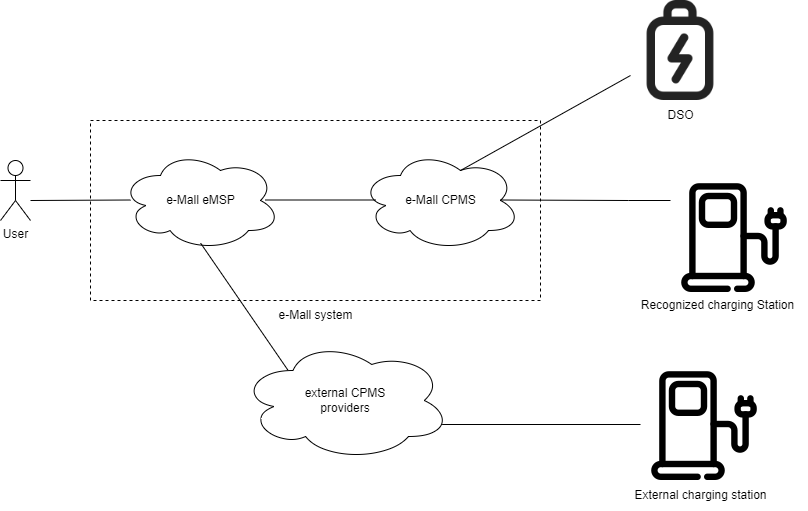
\includegraphics[width=0.70\textwidth]{assets/highest_level_system.drawio.png}
    \caption{High level overview of the e-Mall system}
    %%\label{fig:my_label}
\end{figure} 

\clearpage
\begin{figure}[h]
    \centering
    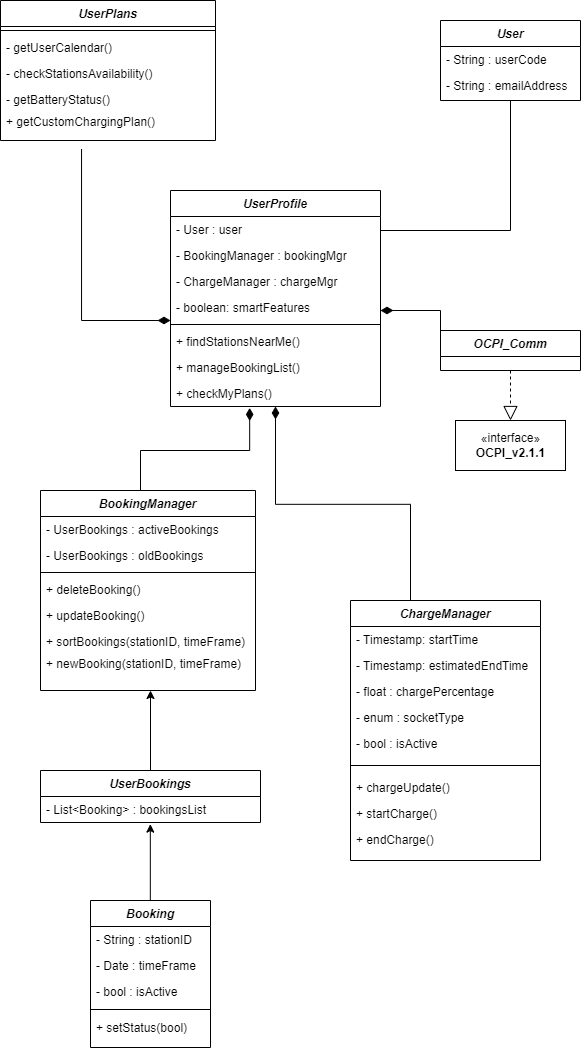
\includegraphics[width = 0.75\textwidth]{assets/e-Mall EMSP.drawio (1).png}
    \caption{Class diagram of the e-Mall eMSP main components}
    \label{fig:my_label}
\end{figure}
\clearpage
\begin{figure}[h]
    \centering
    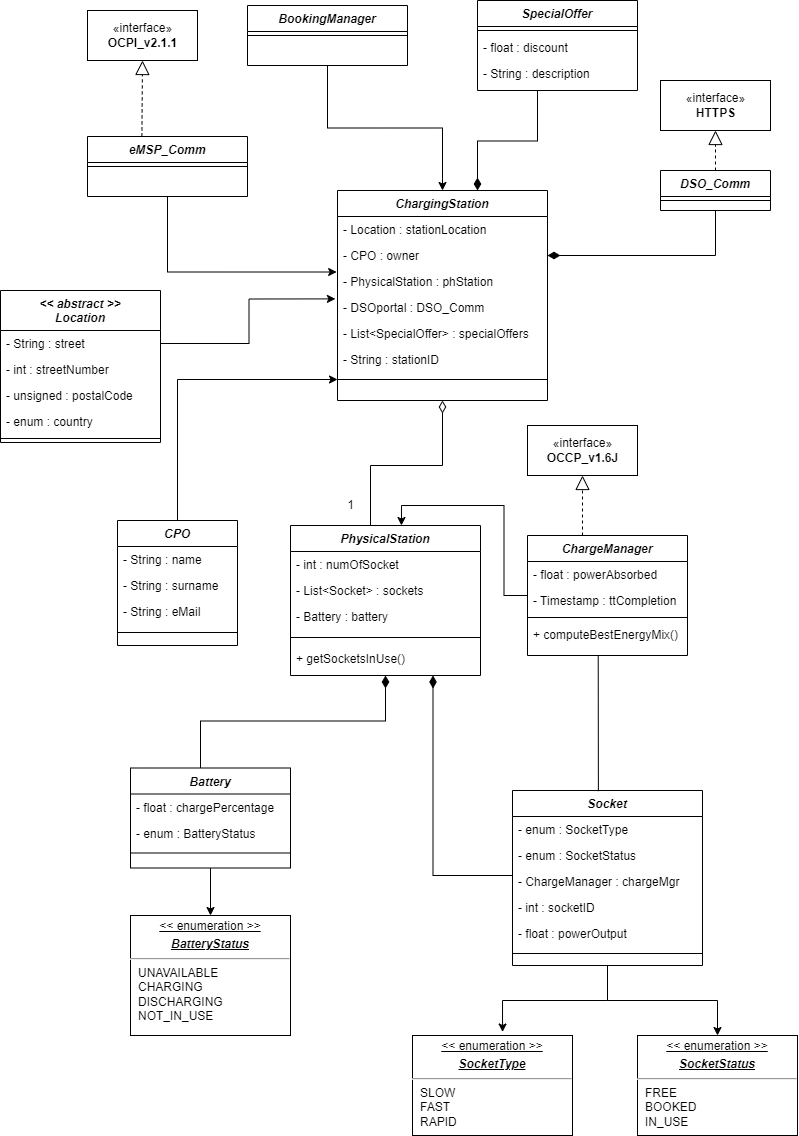
\includegraphics[width = 0.95\textwidth]{assets/e-Mall CPMS.drawio (1).png}
    \caption{Class diagram of the e-Mall CPMS main components}
    \label{fig:my_label}
\end{figure}
\clearpage

\subsection{Activity Diagrams}
This section focuses on the evolution of the system during its interaction with the actors.\\
The activity diagram below shows the interaction between the user and the eMSP, highlighting how the user can book a charge, manage it and see its custom plans based on the daily schedule.

\bigskip

    \begin{figure}[h]
        \centering
        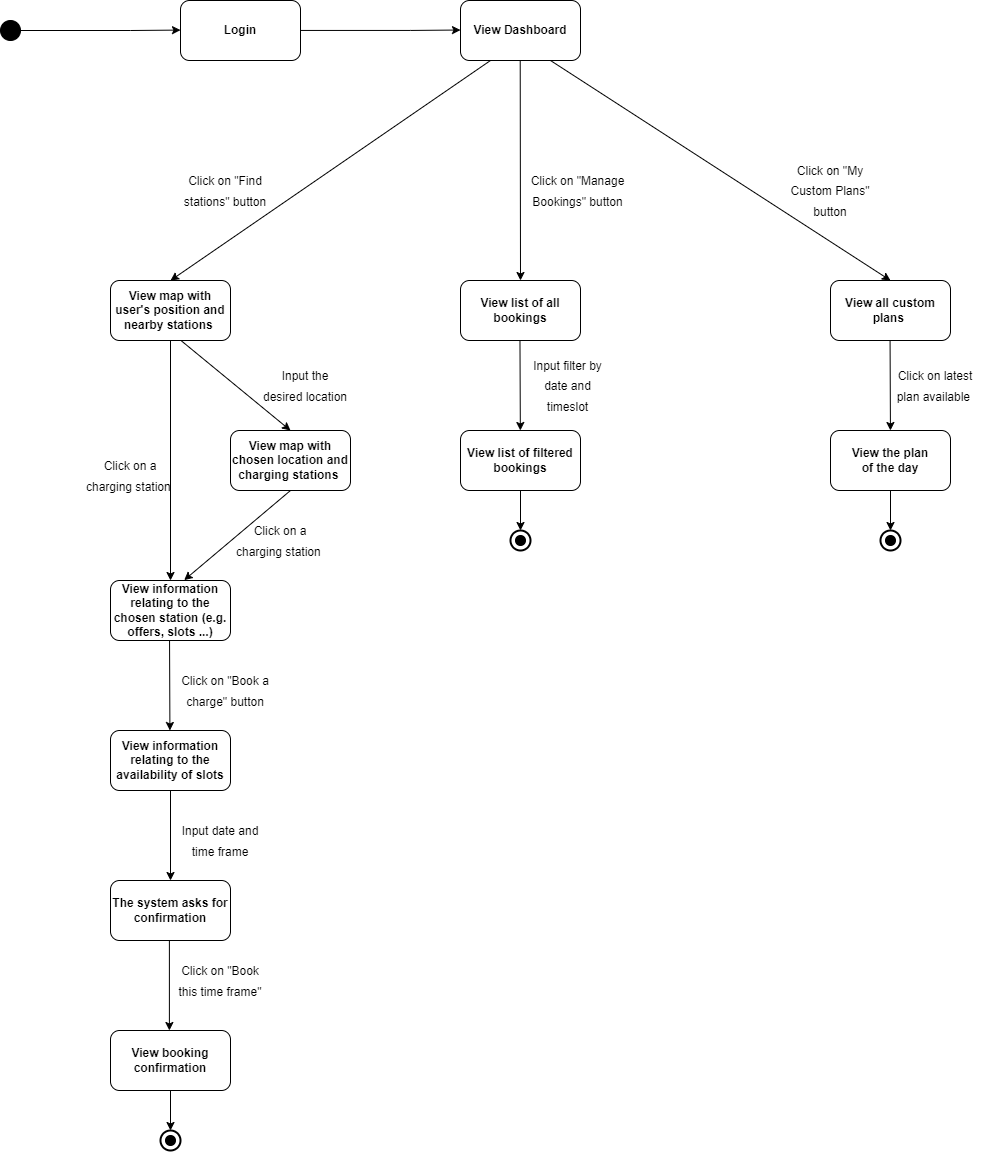
\includegraphics[width=0.88\textwidth]{assets/activitydiagram1.png}
        \caption{User's activity diagram}
        %%\label{fig:my_label}
    \end{figure}
\clearpage
\noindent The activity diagram below shows the interaction between the CPO operator and their Charging Station (through the use of e-Mall CPMS), external DSOs and e-Mall eMSP.

\bigskip

\begin{figure}[h]
    \centering
    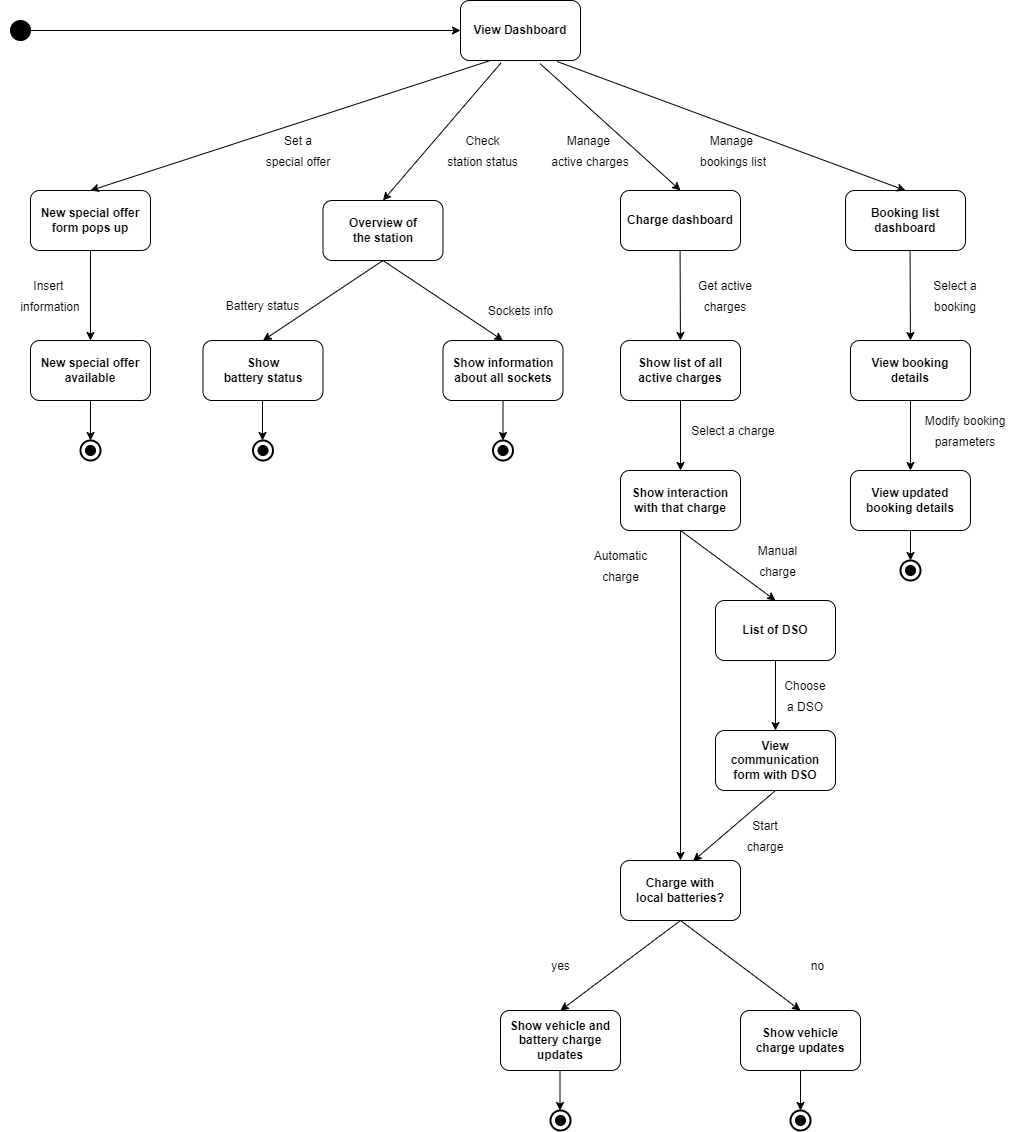
\includegraphics[width=0.88\textwidth]{assets/activitydiagram2.png}
    \caption{CPO's activity diagram}
        %%\label{fig:my_label}
\end{figure}
\newpage

\section{Product Functions}
The aim of the e-Mall system is to provide a platform to combine useful data, involving stations prices, locations, special offers and energy prices for Users, as well as provide CPOs the easiest and most reliable Charging Station handling software. This section presents the main functionalities provided by the e-Mall system.\\
The two main actors are Users and Charging Point Operators.

\subsection{Users Related Functions}
\begin{itemize}
    \item F1: e-Mall eMSP can make a custom charging plan, tailored for the specific user. This is made possible by a smart feature that takes into account the user's habits, their charge status, charging station availability and (if possible) special offers available.
    \item F2: e-Mall eMSP provides the user an up-to-date map of their surroundings (acquired via GPS), highlighting charging stations and special offers they may provide.
    \item F3: e-Mall eMSP provides the user a search bar, to look for charging stations in a specific location.
    \item F4: e-Mall eMSP gives the possibility to show availability in a specific charging station, making it possible to book a specific time slot starting within 15 minutes from the moment of the booking
    \item F5: e-Mall eMSP gives the possibility to consult previous bookings, sort them and, if necessary, delete an active one.
    \item F6: e-Mall eMSP makes it possible to manage the charging process, giving the start and end signal to a charge, monitoring the charging process and eventually pay for the charge.
    \item F7: e-Mall eMSP provides a registration and login platform, so that every action needs to be authenticated before execution.
\end{itemize}

\subsection{CPO Related Functions}
\begin{itemize}
    \item F1: e-Mall CPMS gives operators the possibility to look at their station internal status. So, availability of the charging slots, their type, their energy output and their local batteries status.
    \item F2: e-Mall CPMS provides the operators a way to promote new special offers to be seen by eMSPs users.
    \item F3: e-Mall CPMS provides operators a section to manually interact with DSOs to decide the optimal energy mix to be used and/or be stored in local batteries.
    \item F4: e-Mall CPMS provides operators a section to look at bookings for each charging socket.
    \item F5: e-Mall CPMS provdes operators a way to manually interact with each socket, in order to provide all the functions supported by the DIN (or ISO) protocol implemented.
\end{itemize}

\section{User Characteristics}
e-Mall will support these actors in their interaction with the system:
\begin{itemize}
    \item\textbf{Users}: People who interact with the e-Mall eMSP, they actively perform all the main functions that the software needs to provide;
    \item\textbf{External CPMSs}: Software installed by third parties to manage charging stations. E-Mall eMSP will interact with it;
    \item\textbf{CPO operators}: They can work for a CPO and manually interact with DSOs through e-Mall CPMS.
\end{itemize}

\section{Assumptions, Dependencies \& Constraints}
\begin{itemize}
    \item[\textbf{DA1.}]An internet connection is available at all times during the interaction with the system
    \item[\textbf{DA2.}]Every user has an Internet connected device
    \item[\textbf{DA3.}]Every device used by the users has an integrated GPS sensor
    \item[\textbf{DA4.}]GPS is active when the web application is running
    \item[\textbf{DA5.}] APIs of external CPMSs provide reliable information
    \item[\textbf{DA6.}] APIs of DSOs provide reliable information
    \item[\textbf{DA7.}]Every vehicle is correctly paired with the user’s device at all times
    \item[\textbf{DA8.}]External CPMSs use the same communication protocol as e-Mall (OCCP)
    \item[\textbf{DA9.}]E-Mall can read vehicle’s and user’s data
    \item[\textbf{DA10.}]Every station has an Internet connection
    \item[\textbf{DA11.}]CPMS sensors installed by the CPO are always present and reliable
    \item[\textbf{DA12.}]When the time slot for a charge is active, the charging slot is always accessible
\end{itemize}

\chapter{Specific Requirements}
\section{External Interface Requirements}
\subsection{User Interfaces}

The functionalities of the e-Mall eMSP will be provided through a downloadable web application, this implementation allows for easy access and implementation and will be available for both android and iOS.\\
Users will always use their phone to book and manage the charges through the application, optimized for a more “on the go” use.\\

\subsection{CPMS interfaces}
The functionalities of the e-Mall CPMS will be provided with a downloadable and installable desktop only web application. 
This will provide CPOs with all the necessary tools to manage the charging station, as well as manual interfaces to interact directly with DSOs and the charging sockets.

 

\subsection{Hardware Interfaces}

A user of the system must have access to a smartphone with a stable internet connection and localization provided via GPS in order to interact with the system.\\
A CPO must have access to the dedicated computer of the charging station, which needs to be properly hooked to all the charging station’s sensors in order to provide the functionalities already discussed.

 

\subsection{Software Interfaces}

E-Mall system relies on external interfaces to provide its functionalities. We will now analyze both of the subsystems.
\begin{itemize}
        \item\textbf{Region Map}: The system uses a public API to provide the different users with a map of the geographical region of interest, with respect to their position and their needs. It will also provide special markers in order to show the position of charging stations;
        \item\textbf{External CPMS}: e-Mall needs to face CPMSs of other providers in order to provide the best and most comprehensive charging option available. This communication is made possible by the communication protocol that will be discussed later;
        \item\textbf{DSOs interfaces}: The system will interact through APIs with energy providers (DSOs) and exchange information about charging prices.
\end{itemize}


\newpage
\subsection{Communication Interfaces}
The two subsystems communicate via the internet with each other and external CPMS, making this distinction invisible to the user.\\
The three main communication protocols in use in the e-Mall system: OCPI, OCCP, DIN/ISO. Each component of the system implements the corresponding protocol and uses it for communication with the environment/other subsystems (both internal and external).\\
e-Mall CPMS is also capable of communicating with DSOs through standardized APIs. The communication protocol implemented is HTTPS.\\

\textbf{OCPI (v 2.1.1)} : The Open Charge Point Interface (OCPI) enables a scalable, automated EV roaming setup between CPOs and eMSPs. It supports authorization, charge point information exchange (including live status updates and transaction events), charge detail record exchange, remote charge point commands and, finally, the exchange of smart-charging commands between parties.\\
It also handles the authorization of the charging session and the handling of the bookings.
\begin{figure}[h]
    \centering
    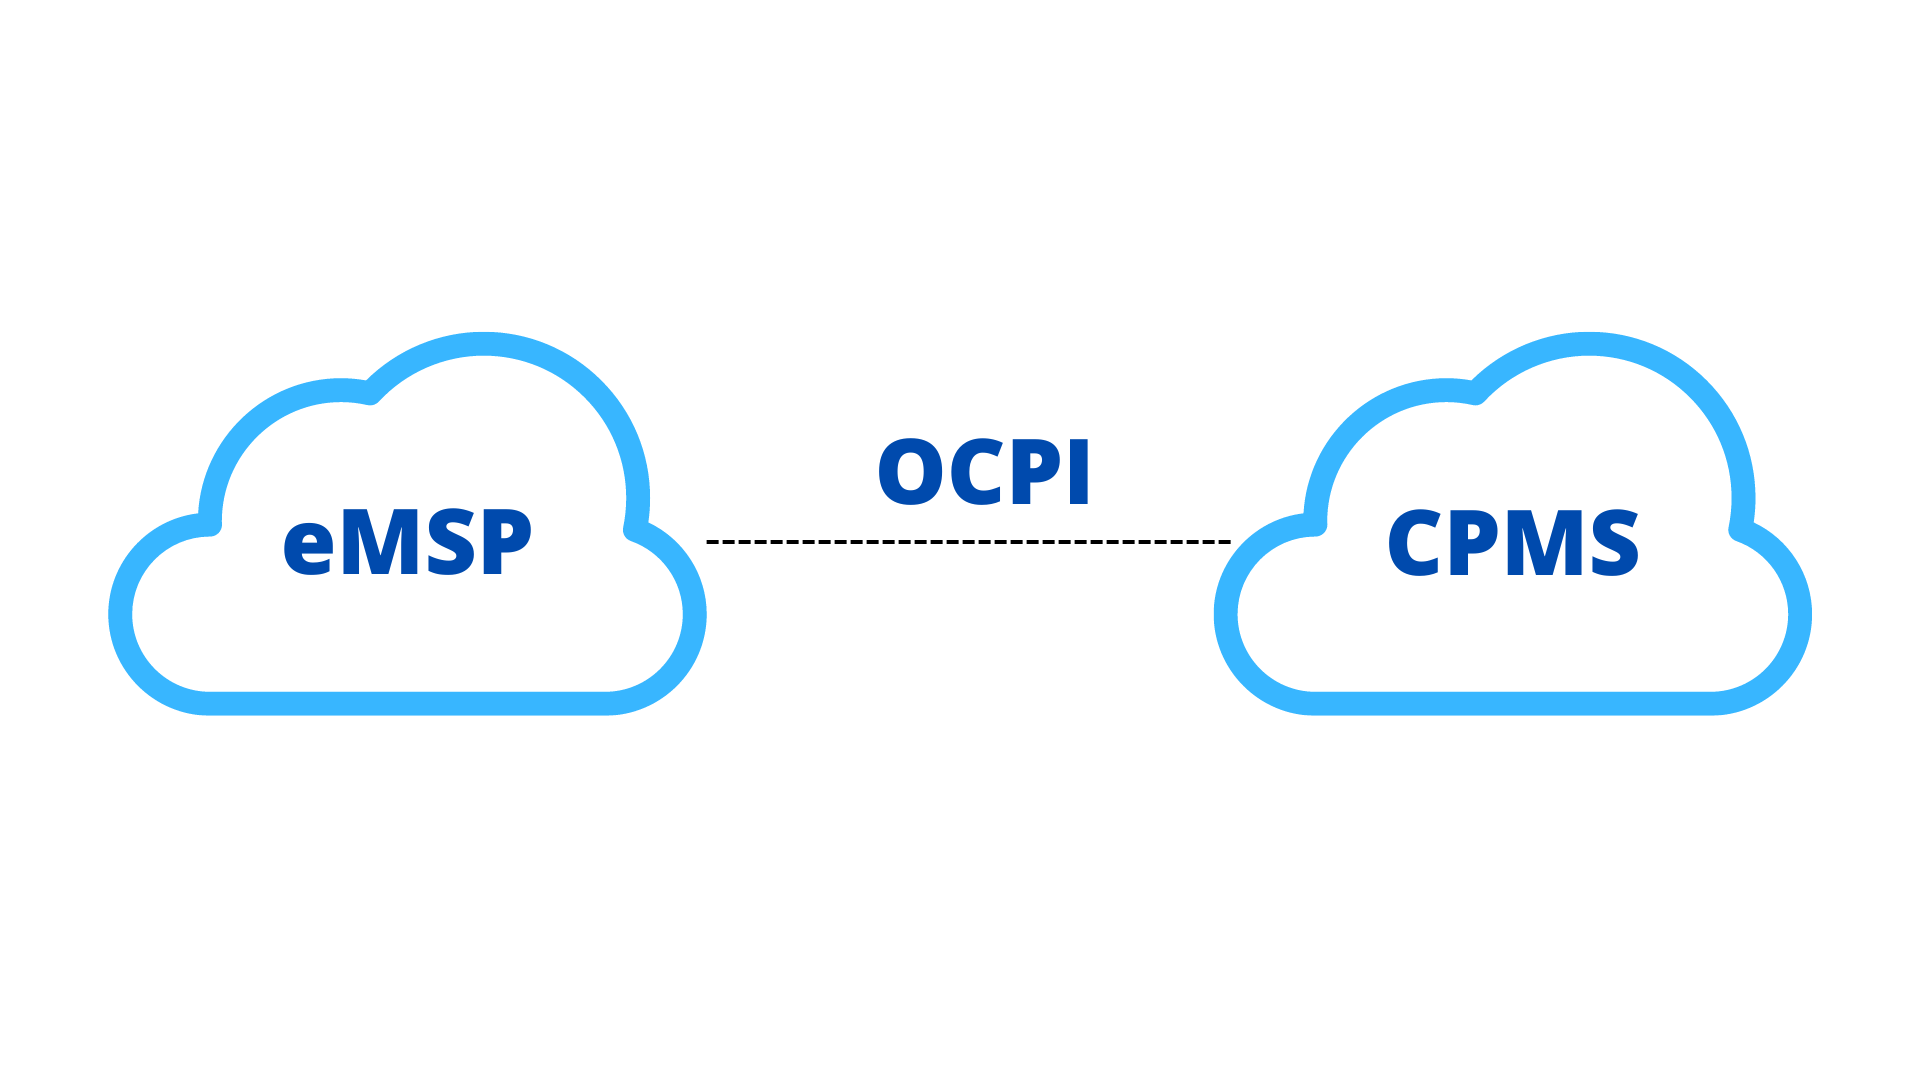
\includegraphics[width = 0.6\textwidth]{assets/OCPI.png}
    \caption{OCPI communication protocol}

\end{figure}

\textbf{OCPP (v 1.6J)} : Communication protocol implemented by CPMS (e-Mall CPMS and external ones). Built on the client-server paradigm, the protocol is used to handle:
    \begin{itemize}
        \item Charging session (Start/Stop session);
        \item Exchange of session data (battery percentage, time left to end the charge, local energy storage status etc.);
        \item Diagnostic of the charging point (reboot, firmware updates, logs);
        \item Updating of the charging point status.
     \end{itemize}
\begin{figure}[h]
    \centering
    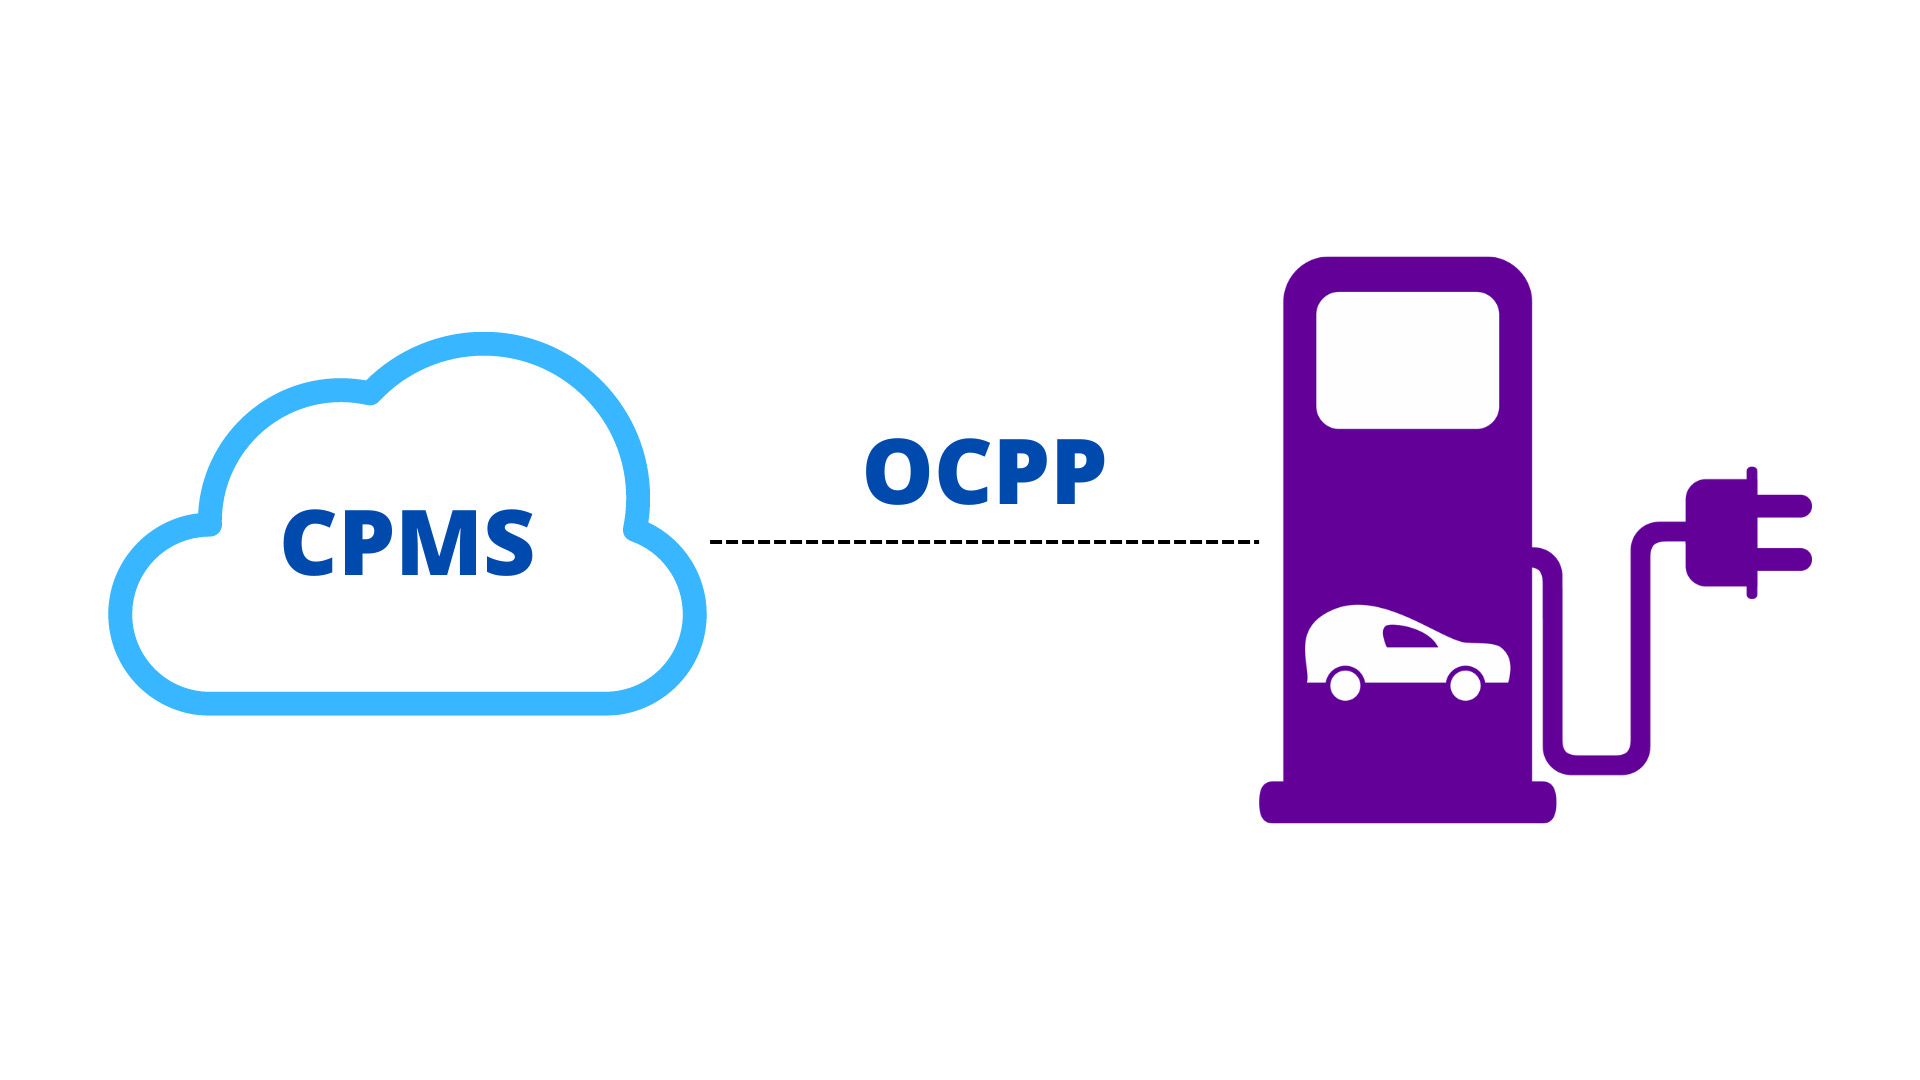
\includegraphics[width = 0.6\textwidth]{assets/OCCP.JPEG}
    \caption{OCPP communication protocol}
\end{figure}
\newpage

\textbf{DIN (SPEC 70121) (or ISO 15118)} : Communication protocol implemented by the CPMSs and some electric vehicles. It handles the exchange of charging information from the vehicle to the CPMS such as:
\begin{itemize}
    \item Electric Vehicle information;
    \item Charging control signal (state of the charge, max power input).
\end{itemize}
In case ISO 15118 is implemented, it can also provide the Plug \& Charge functionality that  enables an electric vehicle to automatically identify and authorize itself to a compatible charging station on behalf of the driver, to receive energy for recharging its battery.
\begin{figure}[h]
    \centering
    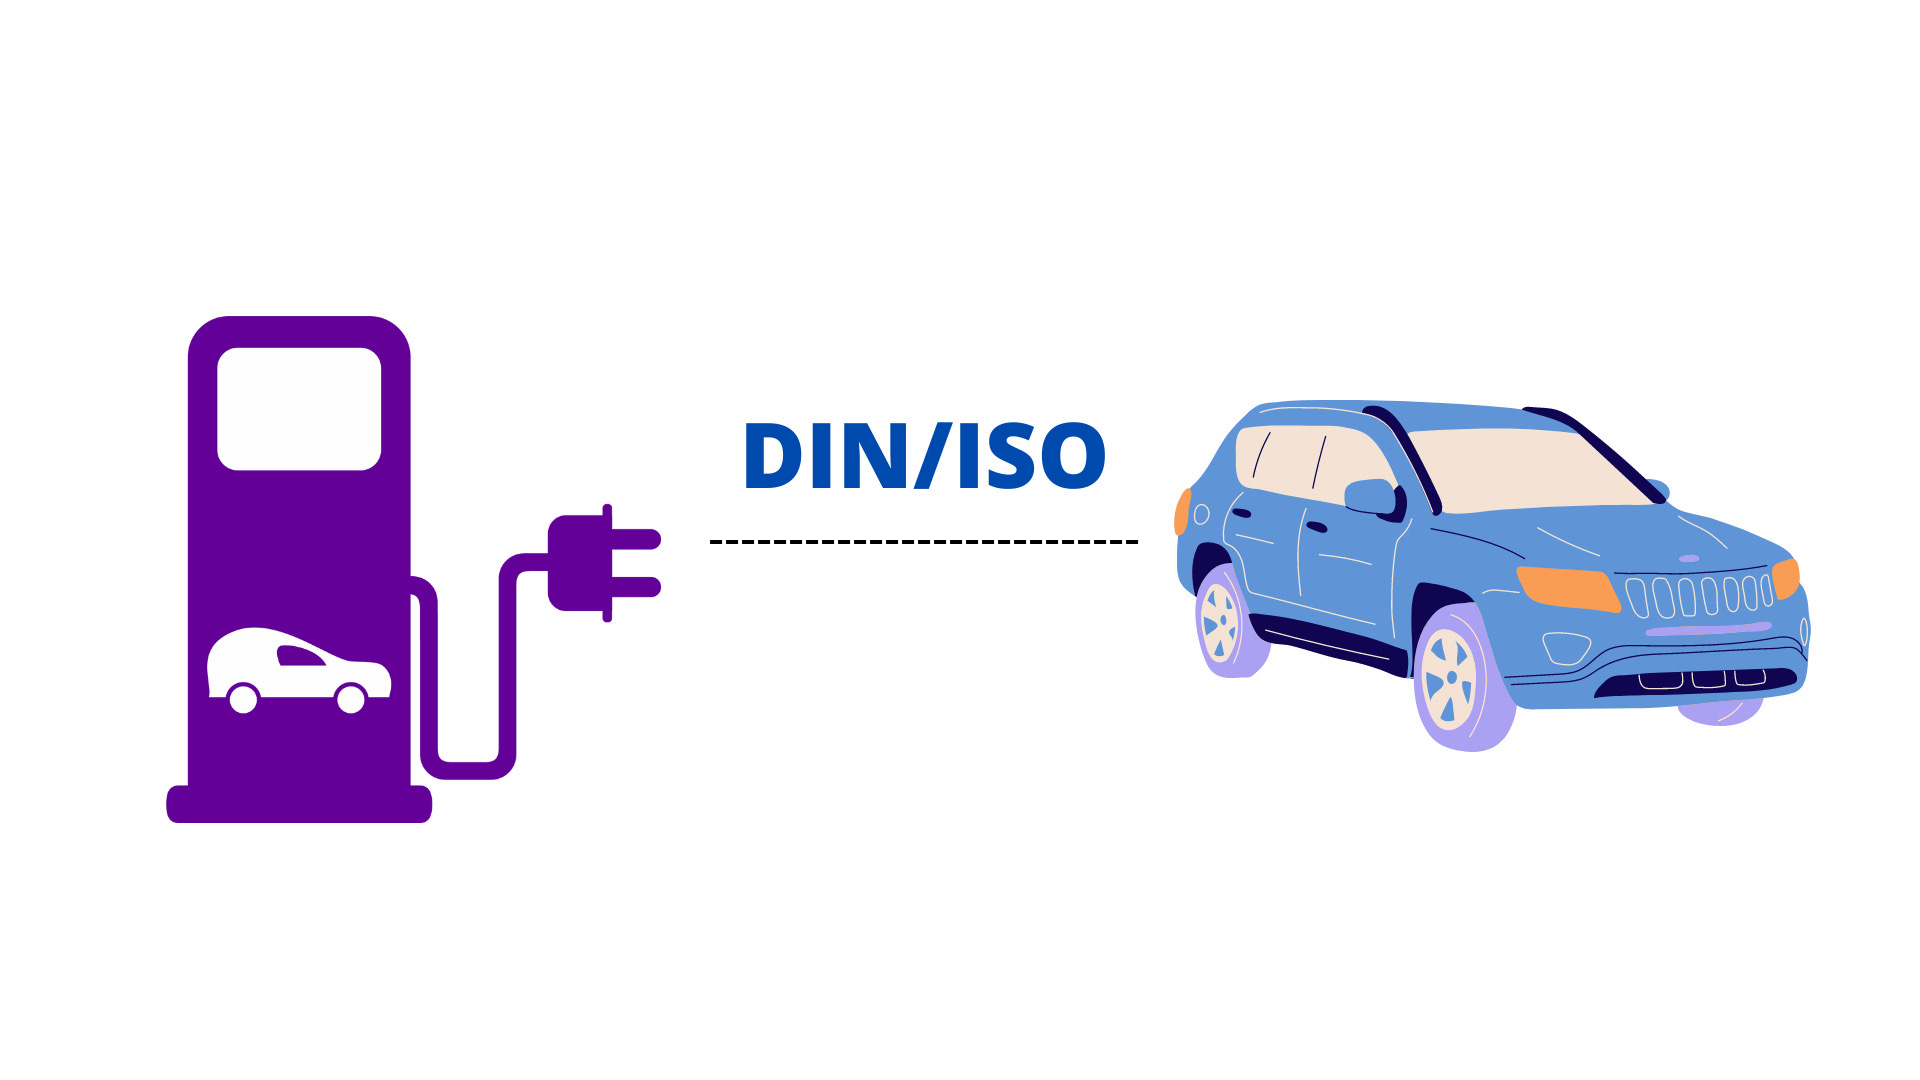
\includegraphics[width = 0.6\textwidth]{assets/DIN-ISO.JPEG}
    \caption{DIN/ISO communication protocols}
\end{figure}

\bigskip

\textbf{Communication Approach}\\
The communication style implemented depends on the communication scenario/interface.\\
\begin{itemize}
    \item\textbf{e-Mall eMSP $\longleftrightarrow$ CPMS}: This scenario requires a mixed communication style.\\The data requests from eMSP to CPMS are performed whenever an user needs for example a rendering of information about stations. In this case a query is performed to nearby stations in order to provide all necessary information. For this reason the system needs to be responsive to asynchronous requests from outside.\\
    When a charge is in progress and updates are provided to the user's eMSP, a series of synchronous messages are exchanged between the parties, as long as the charge is underway. In this case a preferred refresh rate would be 1 update each 3 seconds, taking into consideration the nature of the information that's being exchanged.
    \item\textbf{e-Mall CPMS $\longleftrightarrow$ DSO}: This is a different communication interface, however the communication choice implemented is still asynchronous.\\
    APIs of DSOs are queried when a charge needs to take place and energy prices and sources are required. 
\end{itemize}
\newpage

\section{Functional Requirements}
\subsection{Requirements}
\begin{itemize}
\item[\textbf{R1.}]The e-Mall application should allow users to register by providing their email address


\item[\textbf{R2.}]The e-Mall application should allow users to login using the credentials input at registration time

\item[\textbf{R3.}]The e-Mall application should retrieve locations of charging stations from their CPMS

\item[\textbf{R4.}]The e-Mall application should show availability of charging stations from their CPMS

\item[\textbf{R5.}]The e-Mall application should retrieve prices of charging stations from their CPMS

\item[\textbf{R6.}]The e-Mall application should retrieve special offers of charging stations from their CPMS

\item[\textbf{R7.}]The e-Mall application should acquire locations of charging stations from their CPMS

\item[\textbf{R8.}]The e-Mall application should allow the user to book a charging station for a specific location and time frame

\item[\textbf{R9.}]The e-Mall application should allow the user to delete a previously booked charging station

\item[\textbf{R10.}]The e-Mall application should register a start signal when the “start charge” button is pressed

\item[\textbf{R11.}]The e-Mall application should forward the start signal of the charging to the CPMS 

\item[\textbf{R12.}]The e-Mall application should register an end signal when the “end charge” button is pressed

\item[\textbf{R13.}]The e-Mall application should forward the end signal of the charging to the CPMS

\item[\textbf{R14.}]The e-Mall application should allow users to insert their banking credentials

\item[\textbf{R15.}]The e-Mall application should be able to communicate with the user’s bank

\item[\textbf{R16.}]The e-Mall application should connect to external CPMSs through API

\item[\textbf{R17.}]The e-Mall application should know the charge status of the user’s vehicle

\item[\textbf{R18.}]The e-Mall application should know the daily schedule of the user

\item[\textbf{R19.}]The e-Mall application should be aware of special offers provided by the CPO

\item[\textbf{R20.}]The e-Mall application should be aware of the availability of charging slots at the identified station

\item[\textbf{R21.}]The CPMS should collect real time information about available charging sockets

\item[\textbf{R22.}]The CPMS should collect real time information about the charge speed provided by each charging socket (classified as slow, fast or rapid)

\item[\textbf{R23.}]The CPMS should collect real time information about the cost of a charge

\item[\textbf{R24.}]The CPMS should collect real time information about the estimated time to completion of a charge currently happening

\item[\textbf{R25.}]The CPMS should set an “available” socket as “unavailable” for 15 minutes after it receives a booking

\item[\textbf{R26.}]The CPMS should set a booked socket as “available” if no charge has been started for 15 minutes

\item[\textbf{R27.}]The CPMS should set a booked socket as “available” if the eMSP deletes the relative booking

\item[\textbf{R28.}]The CPMS should set a socket as “unavailable” as long as a charge is in process

\item[\textbf{R29.}]The CPMS should stop dispensing power when the plugged battery is fully charged

\item[\textbf{R30.}]The CPMS should provide real time expenses of a charge

\item[\textbf{R31.}]The CPMS should receive payments from the eMSP

\item[\textbf{R32.}]The CPMS should communicate with DSOs’ API to retrieve the cost of energy

\item[\textbf{R33.}]The CPMS should choose the most convenient DSO based on the eMSPs’ charge requests

\item[\textbf{R34.}]The CPMS should know the CPOs’ local energy availability 

\item[\textbf{R35.}]The CPMS should know if batteries are available in the charging station

\item[\textbf{R36.}]The CPMS should compute where to dispense energy from (local batteries, DSOs or a mixture of the two), to provide the most convenient options

\item[\textbf{R37.}]The CPMS should allow operators to manually handle the energy acquisition and dispense procedure

\item[\textbf{R38.}]The CPMS should communicate the current special offers to the e-Mall application

\item[\textbf{R39.}]The e-Mall application should know the charge status of the user’s vehicle

\item[\textbf{R40.}]The e-Mall application should know the daily schedule of the user

\item[\textbf{R41.}]The e-Mall application should be aware of special offers provided by the CPO

\item[\textbf{R42.}]The e-Mall application should be aware of the availability of charging slots at the identified station
\end{itemize}

\subsection{Mapping of Requirements}
\begin{table}[h]
    \centering
    \begin{tabular}{|c|c|c|c|c|c|c|c|c|c|c|}
        \hline
           & G1 & G2 & G3 & G4 & G5 & G6 & G7 & G8 & G9 & G10\\
        \hline
        DA1&X&X&X&X&X&&&&&\\
        \hline
        DA2&X&X&&&&&&&&\\
        \hline
        DA3&X&X&X&X&&&&&&\\
        \hline
        DA4&X&&&&&&&&&\\
        \hline
        DA5&&&&&X&&&&&X\\
        \hline
        DA6&&&&&&&&&&X\\
        \hline
        DA7&&&&&&X&&&&\\
        \hline
        DA8&&&X&&&&&&&X\\
        \hline
        DA9&&&&&X&&&&&\\
        \hline
        DA10&&&&&&X&&&X&\\
        \hline
        DA11&&&&&&&X&X&&\\
        \hline
        DA12&&&X&X&&X&X&&&\\
        \hline
    \end{tabular}
    \caption{Goal-Domain Assumption mapping}
    \end{table}
\clearpage
\begin{table}[h]
\centering
\begin{tabular}{|c|c|c|c|c|c|c|c|c|c|c|}
\hline
    & G1 & G2 & G3 & G4 & G5 & G6 & G7 & G8 & G9 & G10 \\ \hline
R1  & X  & X  & X  & X  & X  &    &    &    &    &     \\ \hline
R2  & X  & X  & X  & X  & X  &    &    &    &    &     \\ \hline
R3  & X  &    &    &    &    &    &    &    &    &     \\ \hline
R4  & X  &    &    &    &    &    &    &    &    &     \\ \hline
R5  & X  &    &    &    &    &    &    &    &    &     \\ \hline
R6  & X  &    &    &    &    &    &    &    &    &     \\ \hline
R7  & X  &    &    &    &    &    &    &    &    &     \\ \hline
R8  &    & X  &    &    &    &    &    &    &    &     \\ \hline
R9  &    & X  &    &    &    &    &    &    &    &     \\ \hline
R10 &    &    & X  &    &    &    &    &    &    &     \\ \hline
R11 &    &    & X  &    &    &    &    &    &    &     \\ \hline
R12 &    &    & X  &    &    &    &    &    &    &     \\ \hline
R13 &    &    & X  &    &    &    &    &    &    &     \\ \hline
R14 &    &    &    & X  &    &    &    &    &    &     \\ \hline
R15 &    &    &    & X  &    &    &    &    &    &     \\ \hline
R16 &    &    &    &    &    & X  & X  & X  & X  & X   \\ \hline
R17 &    &    &    &    & X  &    &    &    &    &     \\ \hline
R18 &    &    &    &    & X  &    &    &    &    &     \\ \hline
R19 &    &    &    &    & X  &    &    &    &    &     \\ \hline
R20 &    &    &    &    & X  &    &    &    &    &     \\ \hline
R21 &    &    &    &    &    & X  & X  &    &    &     \\ \hline
R22 &    &    &    &    &    & X  & X  &    &    &     \\ \hline
R23 &    &    &    &    &    & X  & X  &    &    &     \\ \hline
R24 &    &    &    &    &    & X  & X  &    &    &     \\ \hline
R25 &    &    &    &    &    &    & X  &    &    &     \\ \hline
R26 &    &    &    &    &    &    & X  &    &    &     \\ \hline
R27 &    &    &    &    &    &    & X  &    &    &     \\ \hline
R28 &    &    &    &    &    &    & X  &    &    &     \\ \hline
R29 &    &    &    &    &    &    & X  &    &    &     \\ \hline
R30 &    &    & X  &    &    &    &    &    & X  &     \\ \hline
R31 &    &    &    &    &    &    &    &    & X  &     \\ \hline
R32 &    &    &    &    &    &    &    &    &    & X   \\ \hline
R33 &    &    &    &    &    & X  &    &    &    &     \\ \hline
R34 &    &    &    &    &    &    &    & X  &    &     \\ \hline
R35 &    &    &    &    &    &    &    & X  &    &     \\ \hline
R36 &    &    &    &    &    &    &    &    &    & X   \\ \hline
R37 &    &    &    &    &    &    &    &    &    & X   \\ \hline
R38 & X  &    &    &    &    & X  &    &    &    &     \\ \hline
R39 &    &    & X  &    & X  &    &    &    &    &     \\ \hline
R40 &    &    &    &    & X  &    &    &    &    &     \\ \hline
R41 & X  &    &    &    &    & X  &    &    &    &     \\ \hline
R42 & X  &    &    &    &    & X  &    &    &    &     \\ \hline
\end{tabular}
\caption{Goal-Requirements mapping}
\end{table}
\clearpage

    \begin{table}[h]
    \centering
    \begin{tabular}{|c|c|c|}
        \hline
         Goal  & Domain Assumptions & Requirements\\
        \hline
        G1 & DA1, DA2, DA3, DA4 & R1, R2, R3, R4, R5, R6, R7, R38, R41, R42\\
        \hline
        G2 & DA1, DA2, DA3 & R1, R2, R8, R9\\
        \hline
        G3 & DA1, DA3, DA8, DA12 & R1, R2, R10, R11, R12, R13, R30, R 39\\
        \hline
        G4 & DA1, DA3, DA12 & R1, R2, R14, R15\\
        \hline
        G5 & DA1, DA5, DA9 & R1, R2, R17, R18, R19, R20, R 39, R40\\
        \hline
        G6 & DA7, DA10, DA12 & R16, R21, R22, R23, R24, R33, R38, R41, R42\\
        \hline
        G7 & DA11, DA12 & R16, R21, R22, R23, R24, R25, R26, R27, R28, R29\\
        \hline
        G8 & DA11 & R16, R34, R35\\
        \hline
        G9 &  DA10 & R16, R30, R31\\
        \hline
        G10 & DA5, DA6, DA8 & R16, R32, R36, R37\\
        \hline
    \end{tabular}
    \caption{Goal-Domain Assumptions-Requirements mapping}
    \end{table}

\noindent To simplify the reading, there is a sum up of the domain assumptions and goals used in the tables of the mappings.
Domain assumptions:
\begin{itemize}
    \item[\textbf{DA1.}]An internet connection is available at all times during the interaction with the system
    \item[\textbf{DA2.}]Every user has an Internet connected device
    \item[\textbf{DA3.}]Every device (smartphone or computer) used by the users has an integrated GPS sensor
    \item[\textbf{DA4.}]GPS is active when the web application is running
    \item[\textbf{DA5.}] APIs of external CPMSs provide reliable information
    \item[\textbf{DA6.}] APIs of DSOs provide reliable information
    \item[\textbf{DA7.}]Every vehicle is correctly paired with the user’s device at all times
    \item[\textbf{DA8.}]External CPMSs use the same communication protocol as e-Mall (OCCP, OCPI)
    \item[\textbf{DA9.}]E-Mall can read vehicle’s and user’s data
    \item[\textbf{DA10.}]Every station has an Internet connection
    \item[\textbf{DA11.}]CPMS sensors installed by the CPO are always 
    present and reliable
    \item[\textbf{DA12.}]When the time slot for a charge is active, the charging slot is always accessible
\end{itemize}
\newpage
\noindent Goals:
\begin{itemize}
\item[\textbf{G1.}]   Allow users to know the location, status, prices and special offers provided by charging stations
\item[\textbf{G2.}]  Allow users to manage bookings of  a charge in a specific location and time frame
\item[\textbf{G3.}] Allow users to start, monitor and end the charging process
\item[\textbf{G4.}] Allow users to pay for the obtained service
\item[\textbf{G5.}] Suggest users to charge their vehicle based on the charge status, the schedule of the users, special offers provided by the CPOs and availability of the charging slots at the identified charging stations
\item[\textbf{G6.}] Provide a complete “external” overview of the charging station (location, availability, charging options…)
\item[\textbf{G7.}] Manage and correctly execute a charge for a specific time frame
\item[\textbf{G8.}] Know the “internal” status of a charging station
\item[\textbf{G9.}] Handle the payment of a charge
\item[\textbf{G10.}] Provide the eMSP with the most convenient charging options by choosing to use locally stored energy or acquire it from DSOs
\end{itemize}
    
\clearpage
\clearpage
\newpage

\subsection{Use Cases Description}  
Use cases capture functional requirements of a system from the outside perspective.\\

    \begin{table}[h]
    \centering
    \begin{tabular}{ |p{4cm}|p{11cm}|  }
        \hline
        \multicolumn{2}{|c|}{\textbf{Platform Login}} \\
        \hline
            \textbf{ID} &  UC.1\\
        \hline
            \textbf{Actors} & User\\
        \hline
            \textbf{Entry Conditions} &
                \begin{itemize}
                    \item The user has access to the e-Mall application
                    \item The application is running on his device
                \end{itemize}\\
        \hline
            \textbf{Event Flow} &
                \begin{enumerate}
                    \item The user launches the e-Mall application
                    \item The user clicks the “Sign Up” button
                    \item The user inserts eMail and password
                    \item The user clicks the “submit” button
                \end{enumerate}\\
        \hline
            \textbf{Exit Conditions} & The user is correctly logged in the system\\
        \hline
            \textbf{Exceptions} &
                \begin{itemize}
                    \item If the userCode is not recognized by the system, the credentials are not registered or the userCode is incorrect. The system notifies the actor and the procedure is aborted.
                    \item If the inserted password is wrong, the system notifies the actor and the procedure is aborted
                \end{itemize}\\
        \hline
    \end{tabular}
    \caption{\label{demo-table}Platform Login use case}
    \end{table}
    

    \clearpage

    \begin{table}[h]
        \centering
        \begin{tabular}{ |p{4cm}|p{11cm}|  }
        \hline
        \multicolumn{2}{|c|}{\textbf{Stations Check In A Specified Location}} \\
        \hline
            \textbf{ID} &  UC.2\\
        \hline
            \textbf{Actors} & User\\
        \hline
            \textbf{Entry Conditions} &
                \begin{itemize}
                    \item The user has accessed the e-Mall application
                    \item The application is running on his device
                    \item The GPS is properly set up and working
                    \item The internet connection works properly
                \end{itemize}\\
        \hline
            \textbf{Event Flow} &
                \begin{enumerate}
                    \item The user launches the e-Mall application
                    \item The user selects the “Find Stations" 
                    section
                    \item The user inputs the desired location
                    \item The system show a map marking the charging stations in the area
                \end{enumerate}\\
        \hline
            \textbf{Exit Conditions} & The user is met with a map marking the charging stations in the desired location\\
        \hline
            \textbf{Exceptions} &
                \begin{itemize}
                    \item There are no available station in the specified area
                    \item The internet connection is disrupted
                    \item GPS position cannot be acquired
                \end{itemize}\\
        \hline
        \end{tabular}
        \caption{\label{demo-table}Stations Check use case}
    \end{table}
\clearpage

 \clearpage
    \begin{table}[h]
    \centering
        \begin{adjustbox}{max width=0.89\textwidth}
        \begin{tabular}{ |p{4cm}|p{11cm}|  }
        \hline
        \multicolumn{2}{|c|}{\textbf{Book a Charge}} \\
        \hline
            \textbf{ID} &  UC.3\\
        \hline
            \textbf{Actors} & User\\
        \hline
            \textbf{Entry Conditions} &
                \begin{itemize}
                    \item The user has accessed the e-Mall application
                    \item The application is running on his device
                    \item The GPS is properly set up and working
                    \item The internet connection works properly
                    \item The user has a view of the stations to choose from
                \end{itemize}\\
        \hline
            \textbf{Event Flow} &
                \begin{enumerate}
                    \item The user selects a specific station
                    \item The system shows all details regarding that specific station
                    \item The user goes to the “Book a Charge” page in said station
                    \item The user selects a date and a time frame 
                    \item The user submits the form
                    \item System asks for confirmation
                    \item The user clicks on “Book this time frame”
                    \item The system shows the booking to the user
                    \item The system notifies the user using the provided contacts
                \end{enumerate}\\
        \hline
            \textbf{Exit Conditions} & 
                \begin{itemize}
                    \item The user has correctly booked a charge in a specific station and time frame
                    \item The charge has been added to the section “My Bookings” in the user’s profile
                \end{itemize}\\
        \hline
            \textbf{Exceptions} &
                \begin{itemize}
                    \item The internet connection is disrupted
                    \item The time frame selected has been taken by another user before the system receives a confirmation from current user
                    \item GPS position cannot be acquired
                \end{itemize}\\
        \hline
        \end{tabular}
        \end{adjustbox}
        \caption{\label{demo-table}Book a Charge use case}
    \end{table}
\clearpage

    \newpage
    \begin{table}[h]
        \centering
        \begin{tabular}{ |p{4cm}|p{11cm}|  }
        \hline
        \multicolumn{2}{|c|}{\textbf{Monitor Booking}} \\
        \hline
            \textbf{ID} &  UC.4\\
        \hline
            \textbf{Actors} & User\\
        \hline
            \textbf{Entry Conditions} &
                \begin{itemize}
                    \item The user has accessed the e-Mall application
                    \item The application is running on his device
                \end{itemize}\\
        \hline
            \textbf{Event Flow} &
                \begin{enumerate}
                    \item The user goes to the "Manage bookings list" section
                    \item The user can filter bookings by date and time slot
                    \item The system provides the user a list with all the bookings that match the filter
                \end{enumerate}\\
        \hline
            \textbf{Exit Conditions} & The user views the bookings\\
        \hline
            \textbf{Exceptions} & If no bookings are available, an error is prompted\\
        \hline
        \end{tabular}
        \caption{\label{demo-table}Monitor Bookings use case}
    \end{table}
    \clearpage

    \clearpage
    \begin{table}[h]
        \centering
        \begin{tabular}{ |p{4cm}|p{11cm}|  }
        \hline
        \multicolumn{2}{|c|}{\textbf{Delete Booking}} \\
        \hline
            \textbf{ID} &  UC.5\\
        \hline
            \textbf{Actors} & User\\
        \hline
            \textbf{Entry Conditions} &
                \begin{itemize}
                    \item The user has accessed the e-Mall application
                    \item The application is running on his device
                    \item The user has accessed the “Manage My Booking list” function
                    \item The internet connection works properly
                    \item The charging process for the reservation the user wants to delete didn't started yet
                \end{itemize}\\
        \hline
            \textbf{Event Flow} &
                \begin{enumerate}
                    \item The user sees the reservation they want to delete
                    \item System asks for confirmation
                    \item The user clicks the “Delete” button
                    \item The user confirms the deletion
                    \item The system notifies the user that the deletion process has been successful
                \end{enumerate}\\
        \hline
            \textbf{Exit Conditions} & The selected reservation is deleted from the user’s booking list\\
        \hline
            \textbf{Exceptions} & The internet connection is disrupted\\
        \hline
        \end{tabular}
        \caption{\label{demo-table}Delete Booking use case}
    \end{table}
    \clearpage

    \clearpage
    \begin{table}[h]
        \centering
        \begin{tabular}{ |p{4cm}|p{11cm}|  }
        \hline
        \multicolumn{2}{|c|}{\textbf{Executing a Charge}} \\
        \hline
            \textbf{ID} &  UC.6\\
        \hline
            \textbf{Actors} & User\\
        \hline
            \textbf{Entry Conditions} &
                \begin{itemize}
                    \item The user has accessed the e-Mall application
                    \item The application is running on his device
                    \item The GPS is properly set up and working
                    \item The internet connection works properly
                    \item The vehicle is at the charging station during a booked timeframe
                    \item The plug is inserted in the vehicle
                \end{itemize}\\
        \hline
            \textbf{Event Flow} &
                \begin{enumerate}
                    \item The system sends a notification to the user stating that the booked time frame has started
                    \item The user presses the start button from the application
                    \item The system presents the user with the charging page with the charging percentage and the estimated time to completion, providing updates periodically
                    \item System confirms the end of the charge at the end of time frame or the user decides to stop
                    \item If the user decides to end the charge the system asks for confirmation to end the charge
                \end{enumerate}\\
        \hline
            \textbf{Exit Conditions} & The user has terminated the charging process\\
        \hline
            \textbf{Exceptions} & \\
        \hline
        \end{tabular}
        \caption{\label{demo-table}Executing a Charge use case}
    \end{table}
    \clearpage
    
    \clearpage
    \begin{table}[h]
        \centering
        \begin{tabular}{ |p{4cm}|p{11cm}|  }
        \hline
        \multicolumn{2}{|c|}{\textbf{New Custom Plan}} \\
        \hline
            \textbf{ID} &  UC.7\\
        \hline
            \textbf{Actors} & User\\
        \hline
            \textbf{Entry Conditions} &
                \begin{itemize}
                    \item The user is logged into the application
                    \item e-Mall advanced features are on
                    \item e-Mall has access to user’s calendar
                    \item e-Mall and user’s vehicle are correctly paired
                \end{itemize}\\
        \hline
            \textbf{Event Flow} &
                \begin{enumerate}
                    \item System sends a notification informing the user a new charging plan is available
                    \item User accesses the “My Custom Plans” section in his profile where a list of all custom plans can be checked
                    \item User clicks on the latest one
                \end{enumerate}\\
        \hline
            \textbf{Exit Conditions} & A custom charging plan is available to be read by the users\\
        \hline
            \textbf{Exceptions} & 
                \begin{itemize}
                    \item Permissions have been revoked, so data can’t be collected
                    \item User’s device and vehicle aren’t paired, data can’t be collected
                    \item GPS position cannot be acquired
                \end{itemize}\\
        \hline
        \end{tabular}
        \caption{\label{demo-table}New Custom Plan use case}
    \end{table}
    \clearpage

    \clearpage
    \begin{table}[h]
        \centering
        \begin{tabular}{ |p{4cm}|p{11cm}|  }
        \hline
        \multicolumn{2}{|c|}{\textbf{Request to DSO}} \\
        \hline
            \textbf{ID} &  UC.8\\
        \hline
            \textbf{Actors} & DSO\\
        \hline
            \textbf{Entry Conditions} &
                \begin{itemize}
                    \item Internet connection is available
                    \item DSOs’ API are reachable
                \end{itemize}\\
        \hline
            \textbf{Event Flow} &
                \begin{enumerate}
                    \item e-Mall CPMS connects to the DSO
                    \item e-Mall CPMS requests information about the energy cost and energy mix to the DSO
                    \item DSO provides all information needed
                \end{enumerate}\\
        \hline
            \textbf{Exit Conditions} & Information are available to the e-Mall CPMS\\
        \hline
            \textbf{Exceptions} & Internet connection is disrupted\\
        \hline
        \end{tabular}
        \caption{\label{demo-table}Request to DSO use case}
    \end{table}

    \begin{table}[h]
    \centering
        \begin{tabular}{ |p{4cm}|p{11cm}|  }
        \hline
        \multicolumn{2}{|c|}{\textbf{Exchange Charge Details to DSO}} \\
        \hline
            \textbf{ID} &  UC.9\\
        \hline
            \textbf{Actors} & DSO\\
        \hline
            \textbf{Entry Conditions} &
                \begin{itemize}
                    \item Internet connection is available
                    \item Connection with the DSO is open and running
                \end{itemize}\\
        \hline
            \textbf{Event Flow} &
                \begin{enumerate}
                    \item CPMS requests the DSO to start dispensing energy
                    \item DSO answers with a “start charge” message
                    \item DSO forwards information regarding the charge
                    \item CPMS requests the DSO to stop dispensing energy
                    \item DSO answers with a “stop charge” message
                \end{enumerate}\\
        \hline
            \textbf{Exit Conditions} & Vehicle is fully charged and CPMS has ended the charge process\\
        \hline
            \textbf{Exceptions} & Internet connection is disrupted\\
        \hline
        \end{tabular}
        \caption{\label{demo-table}Exchange Charge Details to DSO use case}
    \end{table}
\clearpage
\newpage
\newpage
\newpage
\newpage
\subsection{Sequence Diagrams}
In this section a series of sequence diagrams is presented, to understand the functioning of the use cases analyzed above.
    
    \begin{figure}[h]
        \centering
        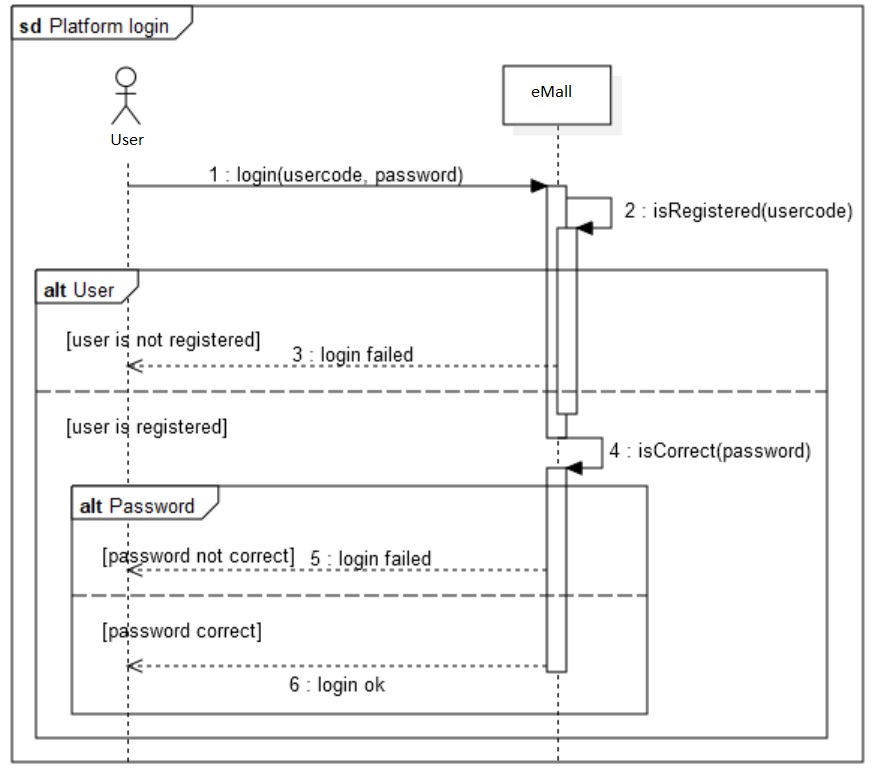
\includegraphics[width=\textwidth]{assets/platform_login.png}
        \caption{Platform Login sequence diagram.}
    \end{figure}
    
    \begin{figure}[h]
        \centering
        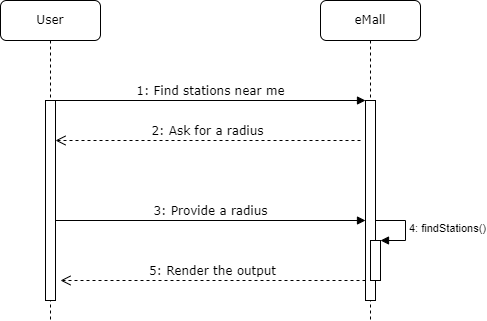
\includegraphics[width=\textwidth]{assets/UC1.png}
        \caption{Stations Check sequence diagram}
    \end{figure}

    \begin{figure}[h]
        \centering
        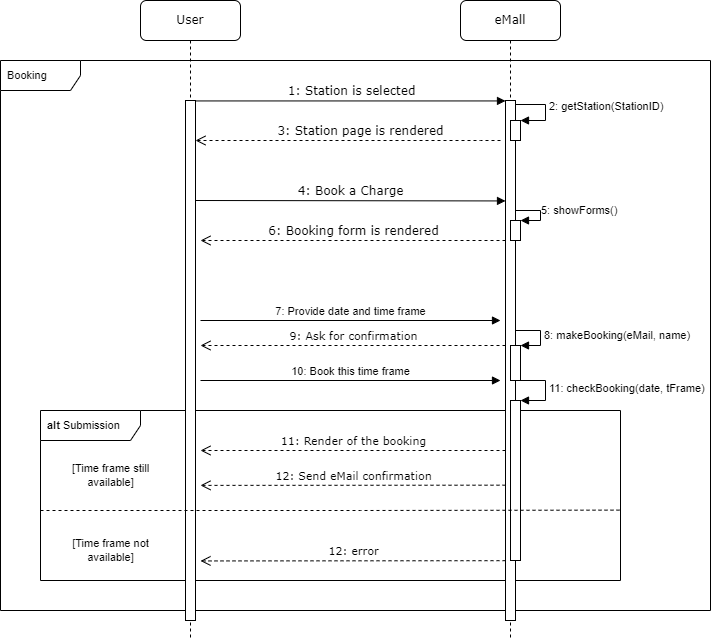
\includegraphics[width=\textwidth]{assets/UC2.drawio.png}
        \caption{Book a Charge sequence diagram}
    \end{figure}

    \begin{figure}[h]
        \centering
        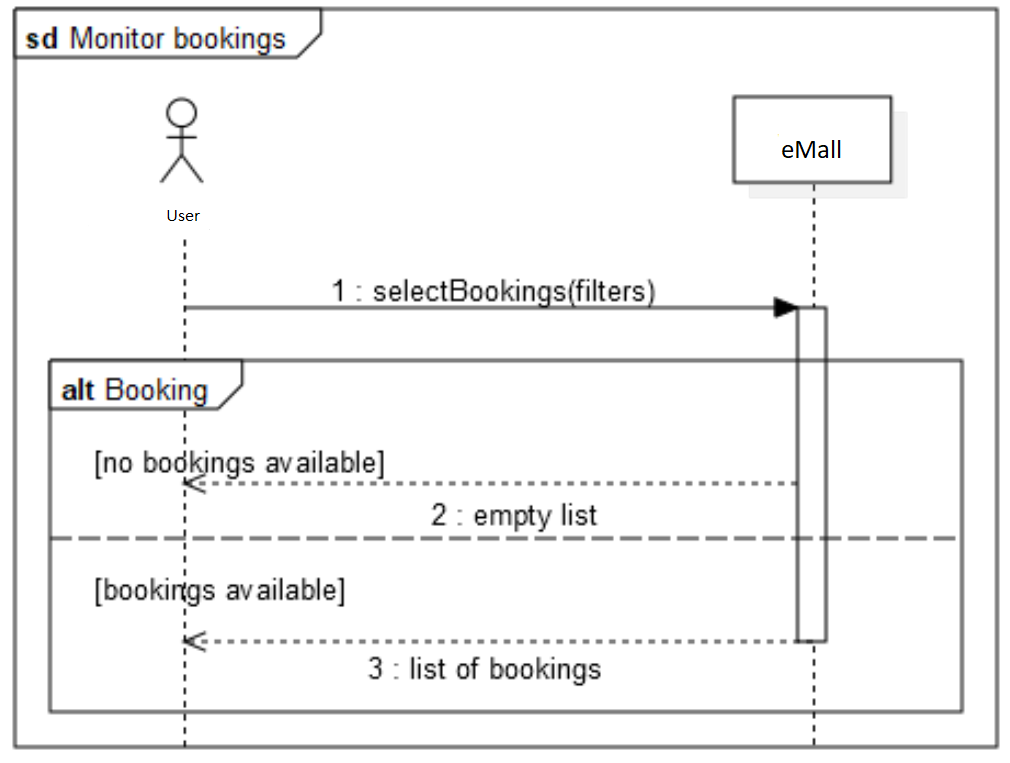
\includegraphics[width=0.7\textwidth]{assets/monitor_booking.png}
        \caption{Monitor Bookings sequence diagram}
    \end{figure}

    \begin{figure}[h]
        \centering
        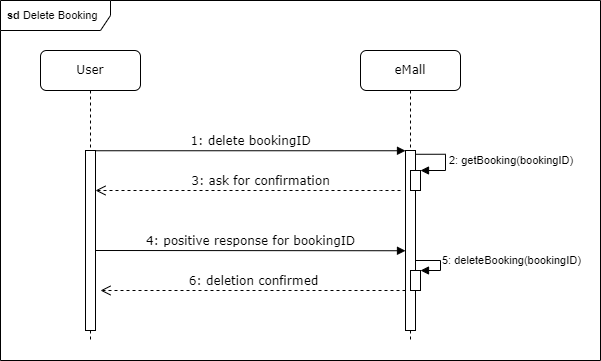
\includegraphics[width=0.8\textwidth]{assets/deletebooking.drawio.png}
        \caption{Delete a Booking sequence diagram}
    \end{figure}

    \begin{figure}[h]
        \centering
        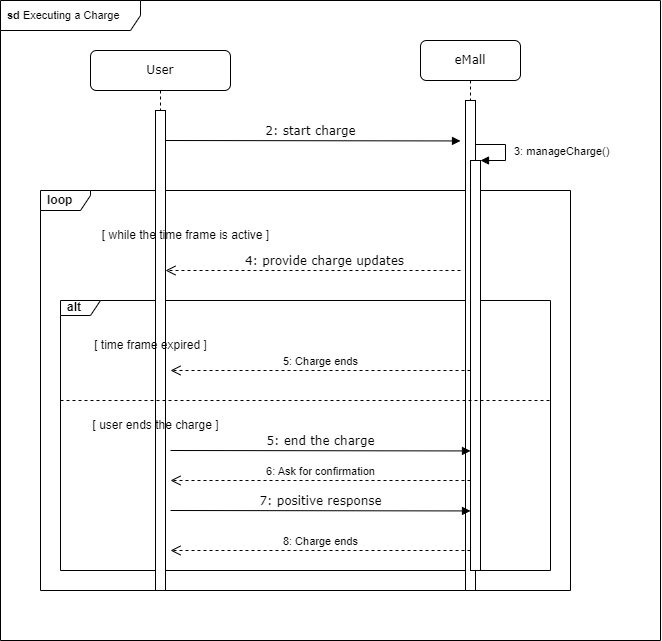
\includegraphics[width=\textwidth]{assets/manage charge.png}
        \caption{Executing a Charge sequence diagram}
    \end{figure}

        \begin{figure}[h]
        \centering
        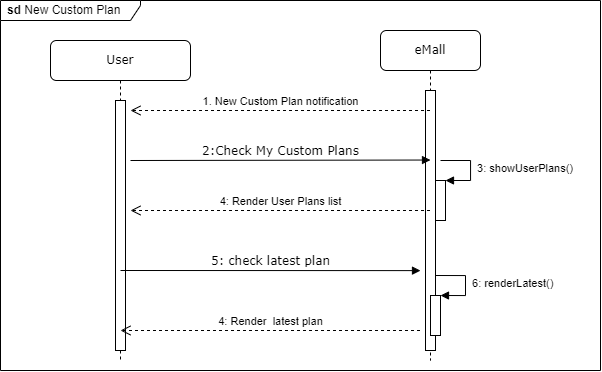
\includegraphics[width=\textwidth]{assets/custom_charge.png}
        \caption{New Custom Plan sequence diagram}
    \end{figure}

    \begin{figure}[h]
        \centering
        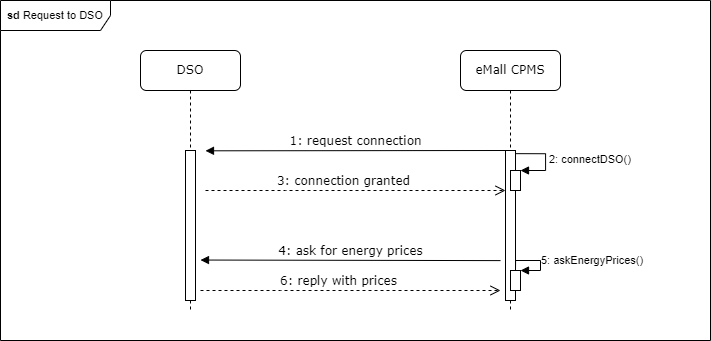
\includegraphics[width = 0.9\textwidth]{assets/request_to_dso.png}
        \caption{Request to DSO sequence diagram}
    \end{figure}

    \begin{figure}
        \centering
        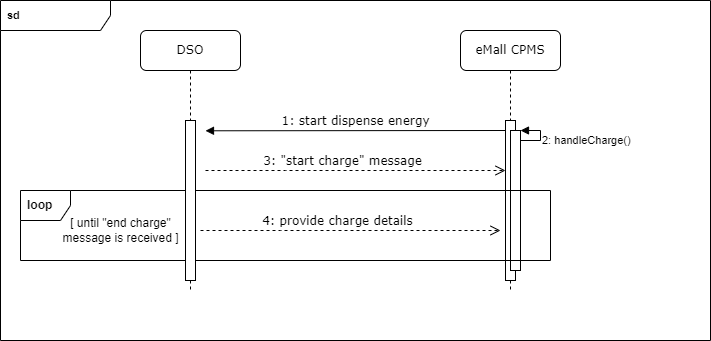
\includegraphics[width = 0.9\textwidth]{assets/exchange_chargr_details_DSO.png}
        \caption{Exchange Charge Details to DSO sequence diagram}
    \end{figure}
\clearpage




\section{Performance Requirements}
The e-Mall application must be able to store data for up to 25.000.000 different users and should be able to support up to 5.000.000 simultaneous connections. This takes into consideration the current number of electric vehicles worldwide, as well as the staggering increase in popularity of renewable energy sources.\\\\
The e-Mall CPMS module must be able to handle at most 500 simultaneous connections. Of course the maximum number of simultaneous charges is equal to the number of sockets provided by the CPO, we estimate it to be by far lower than 500.\\\\
E-Mall eMSP should be able to provide lightweight pages, with a maximum size of 1 MB and a maximum loading time of 5 seconds, in order to overcome possible bottlenecks created by the communication infrastructure.

 
 

\section{Design Constraints}
\subsection{Standards Compliance}
The implementation of the system should follow the requirements stated in this document. It should be well documented in order to facilitate maintenance. Following, the system must manage the procured user data with respect to laws.
\subsection{Hardware Limitations}
The e-Mall application requires the user to own a device capable of connecting to the Internet which also needs GPS which the system must be able to access.
CPOs need to own a desktop computer with the e-Mall eMSP module installed and correctly hooked to the sensors of the station.\\
Moreover, the communication protocols aforementioned need to be conrrectly implemented.
\section{Software System Attributes}
\subsection{Reliability \& Availability}
The system should be the most reliable as possible, this choice is dictated by the frenetic usage of the system that, by nature, is designed for a “on the go” usage.
As mentioned above, the e-Mall system should be a distributed one, in order to provide data consistency and replication. Distributions also allow lower latency for users dislocated in various parts of Europe (main target of the system). Each component of the system should be connected to the Internet 24/7, with sufficient bandwidth to serve all the connected users and sufficient storage to handle all the data involved.
\subsection{Security}
All user information needs to be encrypted, this includes username, password, position and any other information that might be sensitive. The system should be protected against any unauthorized access.
\subsection{Maintainability}
The code of the web application should be written in Java to allow for multi-platform support and agile development of the distributed environment. The code should be well commented and being open source to allow external developers a full comprehension of the internal components.
\subsection{Portability}
Considering the nature of a web application, the e-Mall system should be able to be accessed by mobile users or desktop CPOs.

\chapter{Formal Analysis Using Alloy}
\section{Alloy Model}
Alloy has been used to describe and formally analyze the relationships between the main entities that compose the e-Mall system.
\subsection{Model Description}
The main concepts that were modelled in alloy are: Users, Bookings, Charging Stations, CPOs and CPMSs and all the entities that are useful to specify them.
Then the following constraints were taken into consideration:
\begin{itemize}
    \item Email, Password and UserCode exist only if a User exists
    \item Date exists only if a Booking exists
    \item A TimeSlot exists only if a Booking exists and the start time must be lower than the end time
    \item A Booking exists only if a CPMS exists
    \item An Address exists only if a ChargingStation exists
    \item A ChargingSlot exists only if a ChargingStation exists
    \item A ChargingStation exists only if a CPO exists and it has to have at least one ChargingSlot
    \item A CPMS exists only if a CPO exists
    \item Each User has a unique Email and a unique UserCode
    \item A User can't have two Bookings for the same Date at the same TimeSlot
    \item A Booking belongs to a single CPMS and the ChargingSlot it reserves has to be in a ChargingStation owned by the CPO that has the CPMS to which the Booking belongs
    \item Two Bookings for the same ChargingSlot can't have same Date and overlap in TimeSlots
    \item All CPMS belong to different CPOs
\end{itemize}
\subsection{Alloy Code}
\lstinputlisting[language=alloy]{./assets/e-Mall.als}
\newpage
\section{Metamodels}
In this section, the Metamodels generated to validate some system properties are presented
\subsection{World 1 - General case}
This model shows the entirety of the system and all the complex relations among its part. It's useful to understand how the single parts interact with one another. 
\begin{figure}[h]
    \centering
    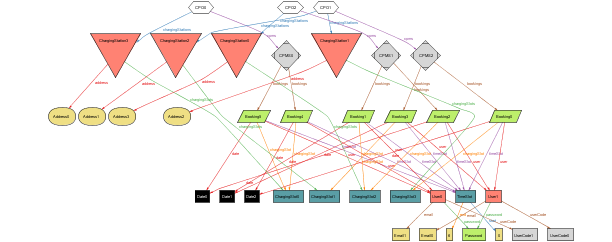
\includegraphics[width = 0.7\textwidth]{assets/alloy_1.png}
    \caption{General World}
\end{figure}

\subsection{World 2 - No overlapping bookings for a station}
For the model generated by the NoOverbooking predicate, it shows the essential property of guaranteeing that no Charging Slot can be booked for more than a customer at the same time. It is clear by the different time slots generated connected to the same date.
\begin{figure}[h]
    \centering
    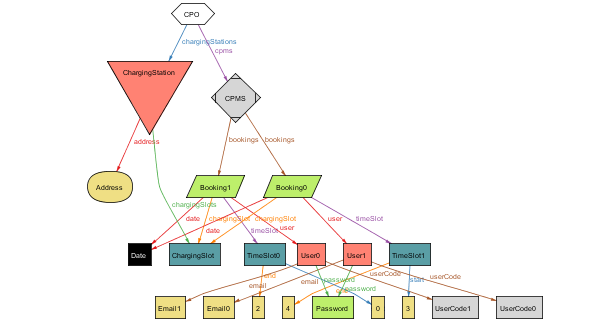
\includegraphics[width = 0.7\textwidth]{assets/alloy_2.png}
    \caption{No overlapping bookings for a station}
\end{figure}
\newpage
\subsection{World 3 - No overlapping bookings for a user}
The diagram shows another fundamental property of the system which is that no user can book more than one charge for the same date and time slot. This is made so to prevent unused reservation, so that the system can be as optimized as possible.
\begin{figure}[h]
    \centering
    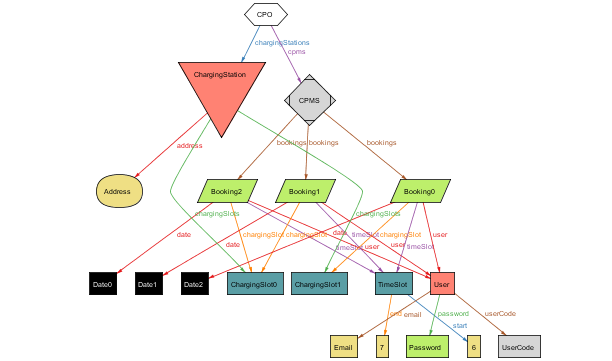
\includegraphics[width = 0.7\textwidth]{assets/alloy_3.png}
    \caption{No overlapping bookings for a user}
\end{figure}

\subsection{World 4 - Charging station with no bookings}
This world shows that a charging station managed by the system developed might not have any bookings. This world was generated to show that the system is compliant even for corner cases such as no bookings for a charging station.
\begin{figure}[h]
    \centering
    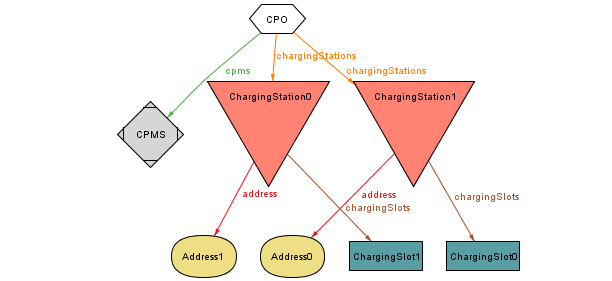
\includegraphics[width = 0.7\textwidth]{assets/alloy_4.png}
    \caption{World with empty charging station}
\end{figure}
\newpage
\subsection{World 5 - User with no bookings}
This world shows that a user might not send any booking request but still be registered in the system. This world was generated to show that the system is compliant even for corner cases such as a registered user that doesn't book any charge.
\begin{figure}[h]
    \centering
    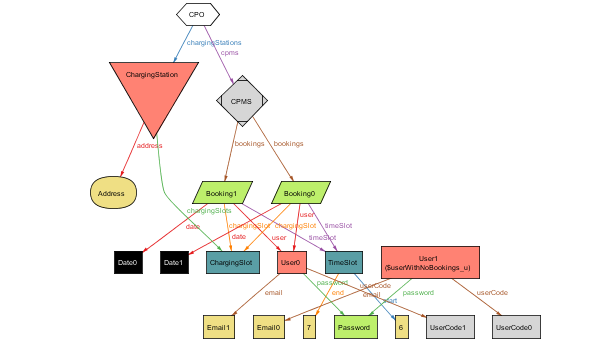
\includegraphics[width = 0.7\textwidth]{assets/alloy_5.png}
    \caption{User with no bookings}
\end{figure}

\newpage
\section{Result of Predicates}
In this section the results of the predicates are shown after running the different worlds of the Alloy model. The result is shown in the Alloy graphical user interface after running the
predicates.
\begin{figure}[h]
    \centering
    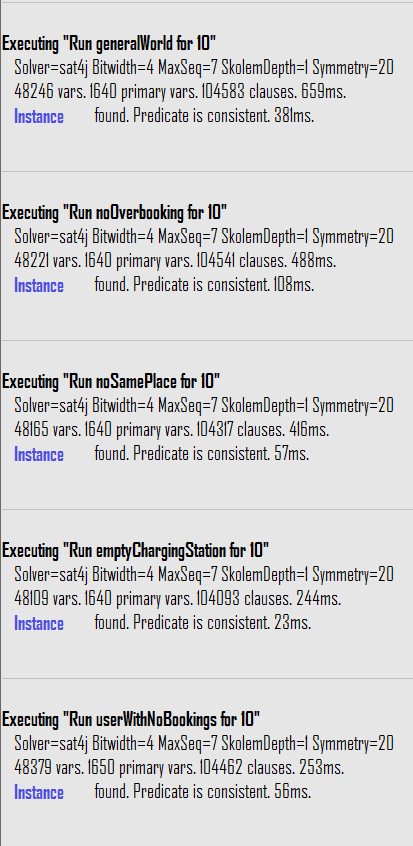
\includegraphics[width = 0.5\textwidth]{assets/alloy_6.png}
    \caption{Result of predicates}
\end{figure}


\chapter{Effort Spent}
\section{Team Effort}
\begin{table}[h]
\centering
\begin{tabular}{lc}
\hline
\multicolumn{1}{|c|}{Task}                                       & \multicolumn{1}{c|}{Time} \\ \hline
\multicolumn{1}{|l|}{Project setup and initial meeting}          & \multicolumn{1}{c|}{3h}    \\ \hline
\multicolumn{1}{|l|}{Introduction}                               & \multicolumn{1}{c|}{1h}    \\ \hline
\multicolumn{1}{|l|}{Domain Assumptions, Goals and Requirements} & \multicolumn{1}{c|}{9h}    \\ \hline
\multicolumn{1}{|l|}{Document Revision}                          & \multicolumn{1}{c|}{9h}    \\ \hline
& \multicolumn{1}{l}{}     
\end{tabular}
\end{table}
\section{Alessia Abbondanza}
\begin{table}[h]
\centering
\begin{tabular}{|l|c|}
\hline
\multicolumn{1}{|c|}{Task}      & Time \\ \hline
Scenarios                       & 1h    \\ \hline
Activity Diagrams               & 3h    \\ \hline
Product Functions               & 3h    \\ \hline
Mapping of Requirements         & 3h    \\ \hline
Use Case Description            & 2h    \\ \hline
Sequence diagrams               & 3h    \\ \hline
Design Constraints              & 2h    \\ \hline
Software System Attributes      & 1h    \\ \hline
Formal Analysis using Alloy     & 6h    \\ \hline
\end{tabular}
\end{table}
\clearpage
\section{Marco Lorenzo Campo}
\begin{table}[h]
\centering
\begin{tabular}{|l|c|}
\hline
\multicolumn{1}{|c|}{Task}      & Time                  \\ \hline
Scenarios                       & 3h                     \\ \hline
Class Diagrams                  & 3h                     \\ \hline
Product Functions               & 2h                     \\ \hline
External Interface Requirements & 4h                     \\ \hline
Mapping of Requirements         & 2h                     \\ \hline
Use Case Description            & 4h                     \\ \hline
Sequence diagrams               & 3h                     \\ \hline
Performance Requirements        & 2h                     \\ \hline
Design Constraints              & 1h                     \\ \hline
Software System Attributes      & 1h \\
\hline
\end{tabular}
\end{table}
\section{Alessandro De Luca}
\begin{table}[h]
\centering
\begin{tabular}{|l|c|}
\hline
\multicolumn{1}{|c|}{Task}      & Time \\ \hline
Scenarios                       & 1h    \\ \hline
Product Functions               & 2h    \\ \hline
Mapping of Requirements         & 2h    \\ \hline
Use Case Description            & 1h    \\ \hline
Performance Requirements        & 1h    \\ \hline
Design Constraints              & 2h    \\ \hline
Software System Attributes      & 1h    \\ \hline
Formal Analysis using Alloy     & 12h   \\ \hline
\end{tabular}
\end{table}



\end{document}
